%% 该模板修改自《计算机学报》latex 模板
%% 主要是将双栏改成单栏,去掉了部分计算机学报标识;
%% 源文件自:https://www.overleaf.com/latex/templates/latextemplet-cjc-xelatex/ybmmymncrrmw
%% 
%%
%% This is file `CjC_template_tex.tex',
%% is modified by Zhi Wang (zhiwang@ieee.org) based on the template 
%% provided by Chinese Journal of Computers (http://cjc.ict.ac.cn/).
%%
%% This version is capable with Overleaf (XeLaTeX).
%%
%% Update date: 2023/03/10
%% -------------------------------------------------------------------
%% Copyright (C) 2016--2023 
%% -------------------------------------------------------------------
%% This file may be distributed and/or modified under the
%% conditions of the LaTeX Project Public License, either version 1.3c
%% of this license or (at your option) any later version.
%% The latest version of this license is in
%%    https://www.latex-project.org/lppl.txt
%% and version 1.3c or later is part of all distribution`s of LaTeX
%% version 2008 or later.
%% -------------------------------------------------------------------

\documentclass[10.5pt,compsoc,UTF8]{CjC}
\usepackage{CTEX}
\usepackage{graphicx}
\usepackage{footmisc}
\usepackage{subfigure}
\usepackage{url}
\usepackage{multirow}
\usepackage{multicol}
\usepackage[noadjust]{cite}
\usepackage{amsmath,amsthm}
\usepackage{amssymb,amsfonts}
\usepackage{booktabs}
\usepackage{color}
\usepackage{ccaption}
\usepackage{booktabs}
\usepackage{float}
\usepackage{fancyhdr}
\usepackage{caption}
\usepackage{xcolor,stfloats}
\usepackage{comment}
\setcounter{page}{1}
\graphicspath{{figures/}}
\usepackage{cuted}%flushend,
\usepackage{captionhack}
\usepackage{epstopdf}
\usepackage{gbt7714}
\usepackage{listings}
\usepackage{xeCJK}
\usepackage{float}
\usepackage{sourcecodepro}
\usepackage[T1]{fontenc}
\usepackage{hyperref}

\setmainfont{Times Roman}
% \setCJKmainfont{Noto Sans Mono CJK TC}
\setCJKmainfont{標楷體.ttc}
\setmonofont{Cascadia Code}

%===============================%

\headevenname{\mbox{\quad} \hfill  \mbox{\zihao{-5}{ \hfill 2024 Hardware Design  } \hspace {50mm} \mbox{2024 年 11 月}}}%
\headoddname{Group 21 \hfill Lab 6: Peripheral Components: VGA, Mouse, and Dual FPGA
}%

%footnote use of *
\renewcommand{\thefootnote}{\fnsymbol{footnote}}
\setcounter{footnote}{0}
\renewcommand\footnotelayout{\zihao{5-}}

\newtheoremstyle{mystyle}{0pt}{0pt}{\normalfont}{1em}{\bf}{}{1em}{}
\theoremstyle{mystyle}
\renewcommand\figurename{figure~}
\renewcommand{\thesubfigure}{(\alph{subfigure})}
\newcommand{\upcite}[1]{\textsuperscript{\cite{#1}}}
\renewcommand{\labelenumi}{(\arabic{enumi})}
\newcommand{\tabincell}[2]{\begin{tabular}{@{}#1@{}}#2\end{tabular}}
\newcommand{\abc}{\color{white}\vrule width 2pt}
\renewcommand{\bibsection}{}
\makeatletter
\renewcommand{\@biblabel}[1]{[#1]\hfill}
\makeatother
\setlength\parindent{2em}
%\renewcommand{\hth}{\begin{CJK*}{UTF8}{gbsn}}
%\renewcommand{\htss}{\begin{CJK*}{UTF8}{gbsn}}
\renewcommand{\contentsname}{Table of Contents}

\begin{document}

\hyphenpenalty=50000
\makeatletter
\newcommand\mysmall{\@setfontsize\mysmall{7}{9.5}}
\newenvironment{tablehere}
  {\def\@captype{table}}

\let\temp\footnote
\renewcommand \footnote[1]{\temp{\zihao{-5}#1}}

\hypersetup{
  colorlinks=false,
  pdfborder={0 0 0},
}

\thispagestyle{plain}%
\thispagestyle{empty}%
\pagestyle{CjCheadings}

% \begin{table*}[!t]
\vspace {-13mm}


\onecolumn
\zihao{5-}\noindent Group 21 \hfill Lab 6: Peripheral Components: VGA, Mouse, and Dual FPGA
 \hfill 2024 年 11 月\\
\noindent\rule[0.25\baselineskip]{\textwidth}{1pt}


\begin{center}
    \vspace {11mm}
    {\zihao{2} \heiti \fangsong Lab 6: Peripheral Components: VGA, Mouse, and Dual FPGA
}
    
    \vskip 5mm
    
    {\zihao{4}\fangsong Group 21: 陳克盈(112062205)、蔡明妡(112062224)}
\end{center}

\lstset{
    % backgroundcolor=\color{red!50!green!50!blue!50},%程式碼塊背景色為淺灰色
    rulesepcolor= \color{gray}, %程式碼塊邊框顏色
    breaklines=true,  %程式碼過長則換行
    numbers=left, %行號在左側顯示
    numberstyle= \small\ttfamily,%行號字型
    keywordstyle= \color{blue},%關鍵字顏色
    commentstyle=\color{gray}, %註釋顏色
    frame=shadowbox%用方框框住程式碼塊
    basicstyle=\ttfamily\footnotesize,
}
 
\definecolor{improvecolor}{rgb}{0,0.6,0} % 深綠色
\definecolor{declinecolor}{rgb}{0.6,0,0} % 深紅色


%%%%%%%%%%%%%%%%%%%%%%%%%%%%%%%%%%%%%%
\zihao{5}
\vskip 10mm
% \begin{multicols}{1}


%%%%%%%%%%%%%%%%%%%%%%%%%%%%%%%%%%%%%%%%%%
%%%%%%%%%%%%%%%%%%%%%%%%%%%%%%%%%%%%%%%%%%

\tableofcontents
\newpage

\section{Chip to Chip}
這題需要補齊 slave 接收與傳送訊號的部分,完成 master 和 slave 之間的溝通協議。
\par
master 會傳送 request,slave 收到 request 後會回傳 ack 給 master,\
master 端接收到 ack 後再將 data 傳送給 slave,\
slave 收到 data 後 decoder 會處理並輸出給 seven\_segment 呈現在板子上。

\begin{figure}[!h]
  \centering
  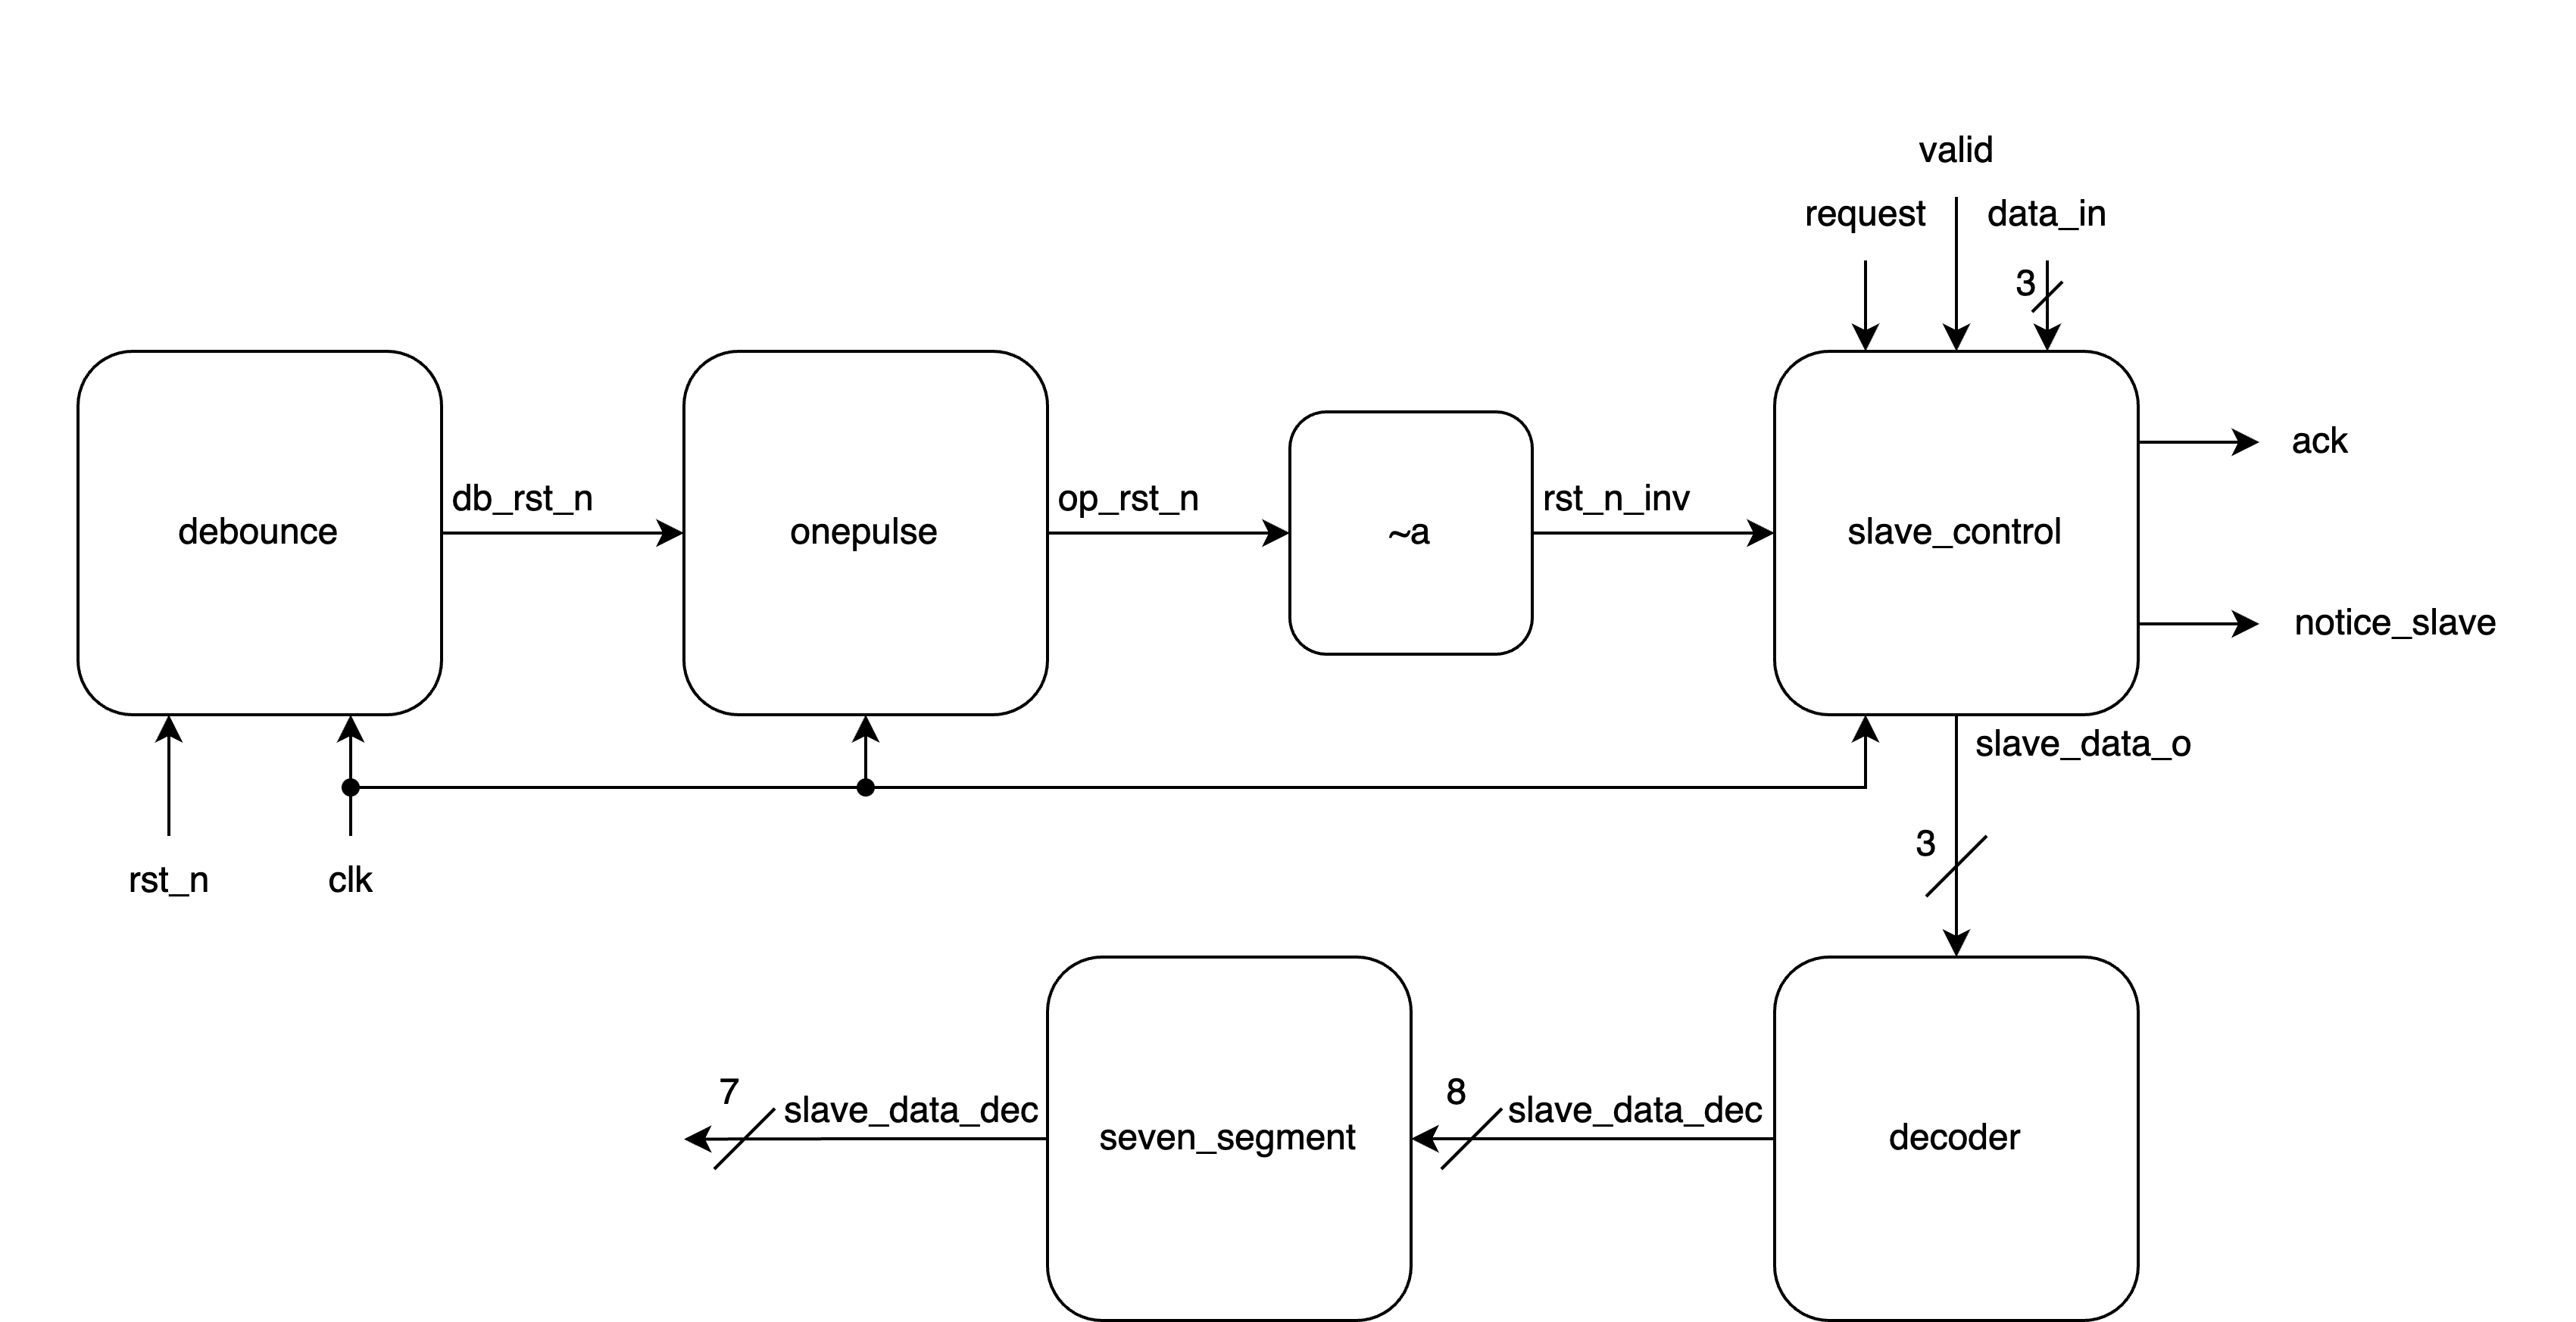
\includegraphics[width=0.9\textwidth]{./img/c2c-1.png}
  \caption{Q1 Slave FPGA block diagram}
  \label{fig:c2c-1}
\end{figure}

對 slave\_control 的 FSM 設計如下:
\begin{itemize}
  \item state\_wait\_rqst:等待 master 傳送 request
  \begin{itemize}
    \item state:收到 master 傳來的 request 後,切換至 state\_wait\_to\_send\_ack
    \item 收到 request 後,切換成 1 開始溝通,此時 counter 會開始運作,\
    直到 count == 27'd100000000 時,將 done 設定為 1
    \item notice:收到 request 後,使 LED[0] 亮起
    \item ack:在這個 state 不做動作保持為 0
    \item data:在這個 state 不做動作保持原本的 data
  \end{itemize}
  \item state\_wait\_to\_send\_ack:等待 done == 1 並且傳送 ack
  \begin{itemize}
    \item state:當 done == 1 時,切換至 state\_wait\_data
    \item start:當 done == 1 時,start 切換回 0 使 counter 停止運作
    \item notice:LED[0] 持續亮起直到 done == 1
    \item ack:當 done == 1 時,將 ack 設成 1 傳送給 master
    \item data:在這個 state 不做動作保持原本的 data
  \end{itemize}
  \item state\_wait\_data:等待 master 傳送 data
  \begin{itemize}
    \item state:收到 master 傳來的 valid 後,切換回 state\_wait\_rqst
    \item start:在這個 state 不做動作保持為 0
    \item notice:在這個 state 不做動作保持為 0
    \item ack:直到收到 master 傳來的 valid 保持為 1
    \item data:收到 valid 後,切換成從 master 傳送來的 data\_in
  \end{itemize}
\end{itemize}

\begin{figure}[!h]
  \centering
  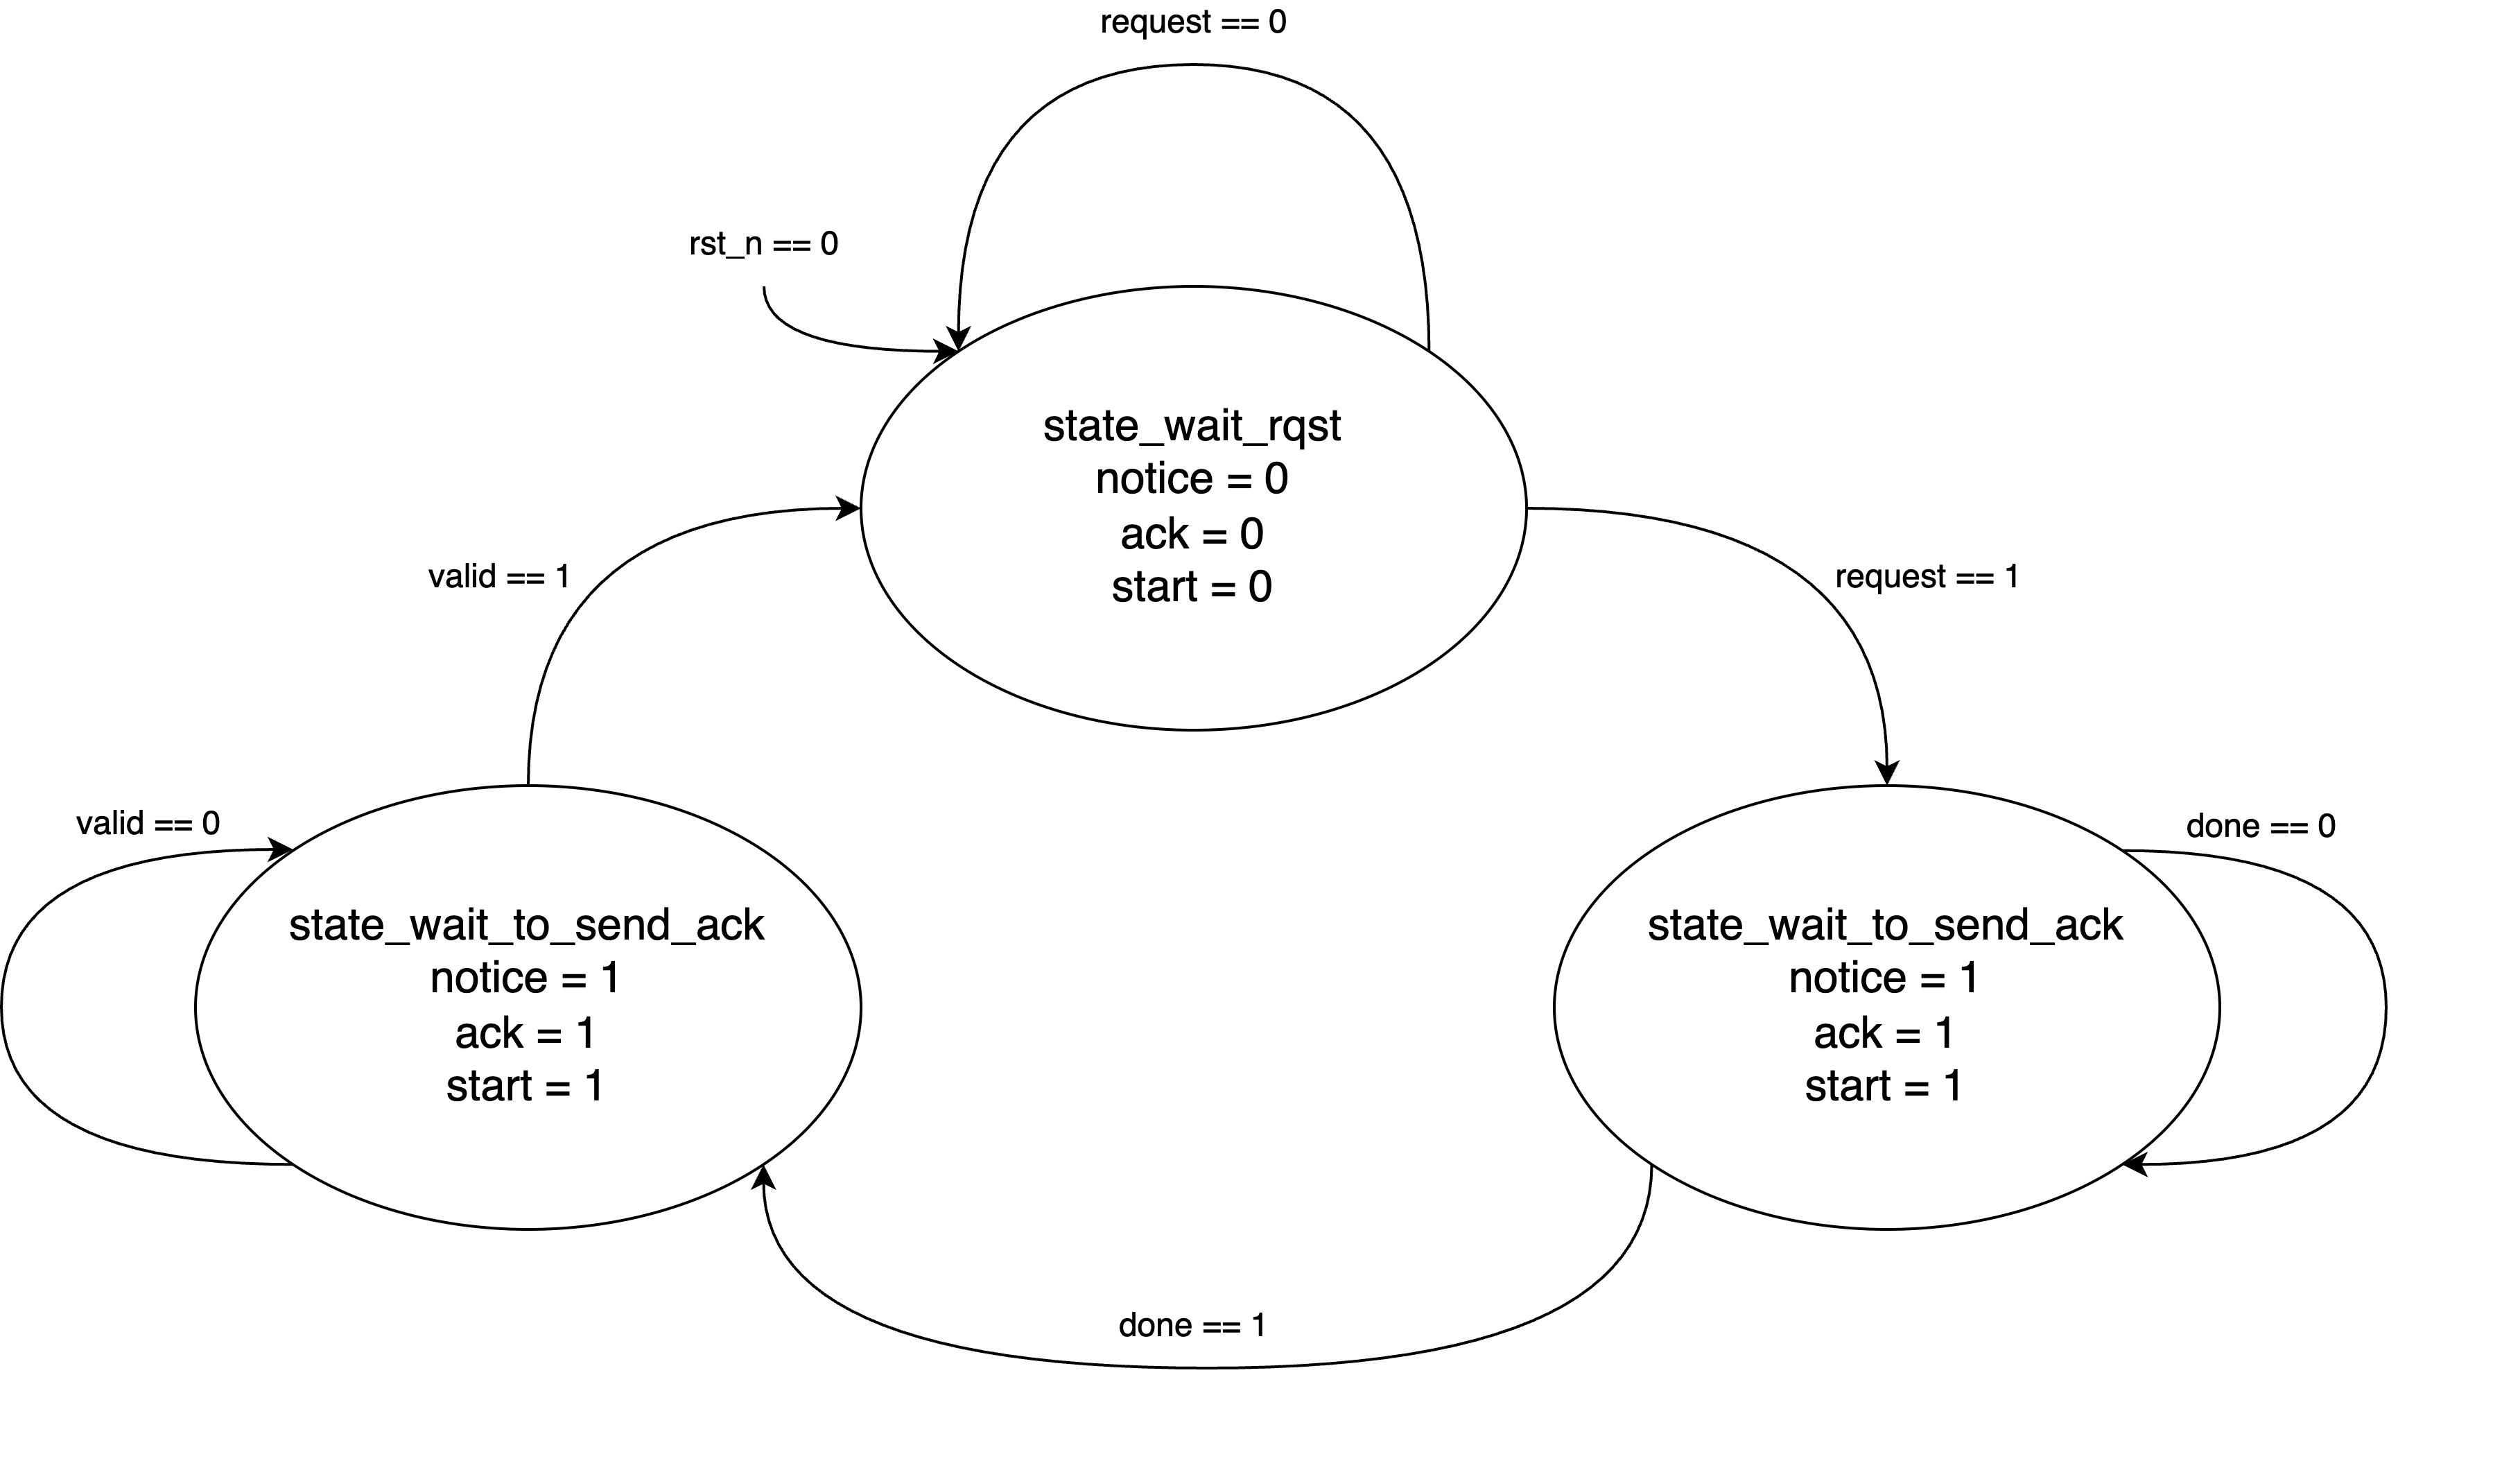
\includegraphics[width=0.9\textwidth]{./img/c2c-2.png}
  \caption{Q1 Slave Control State diagram}
  \label{fig:c2c-2}
\end{figure}

\begin{figure}[!h]
  \centering
  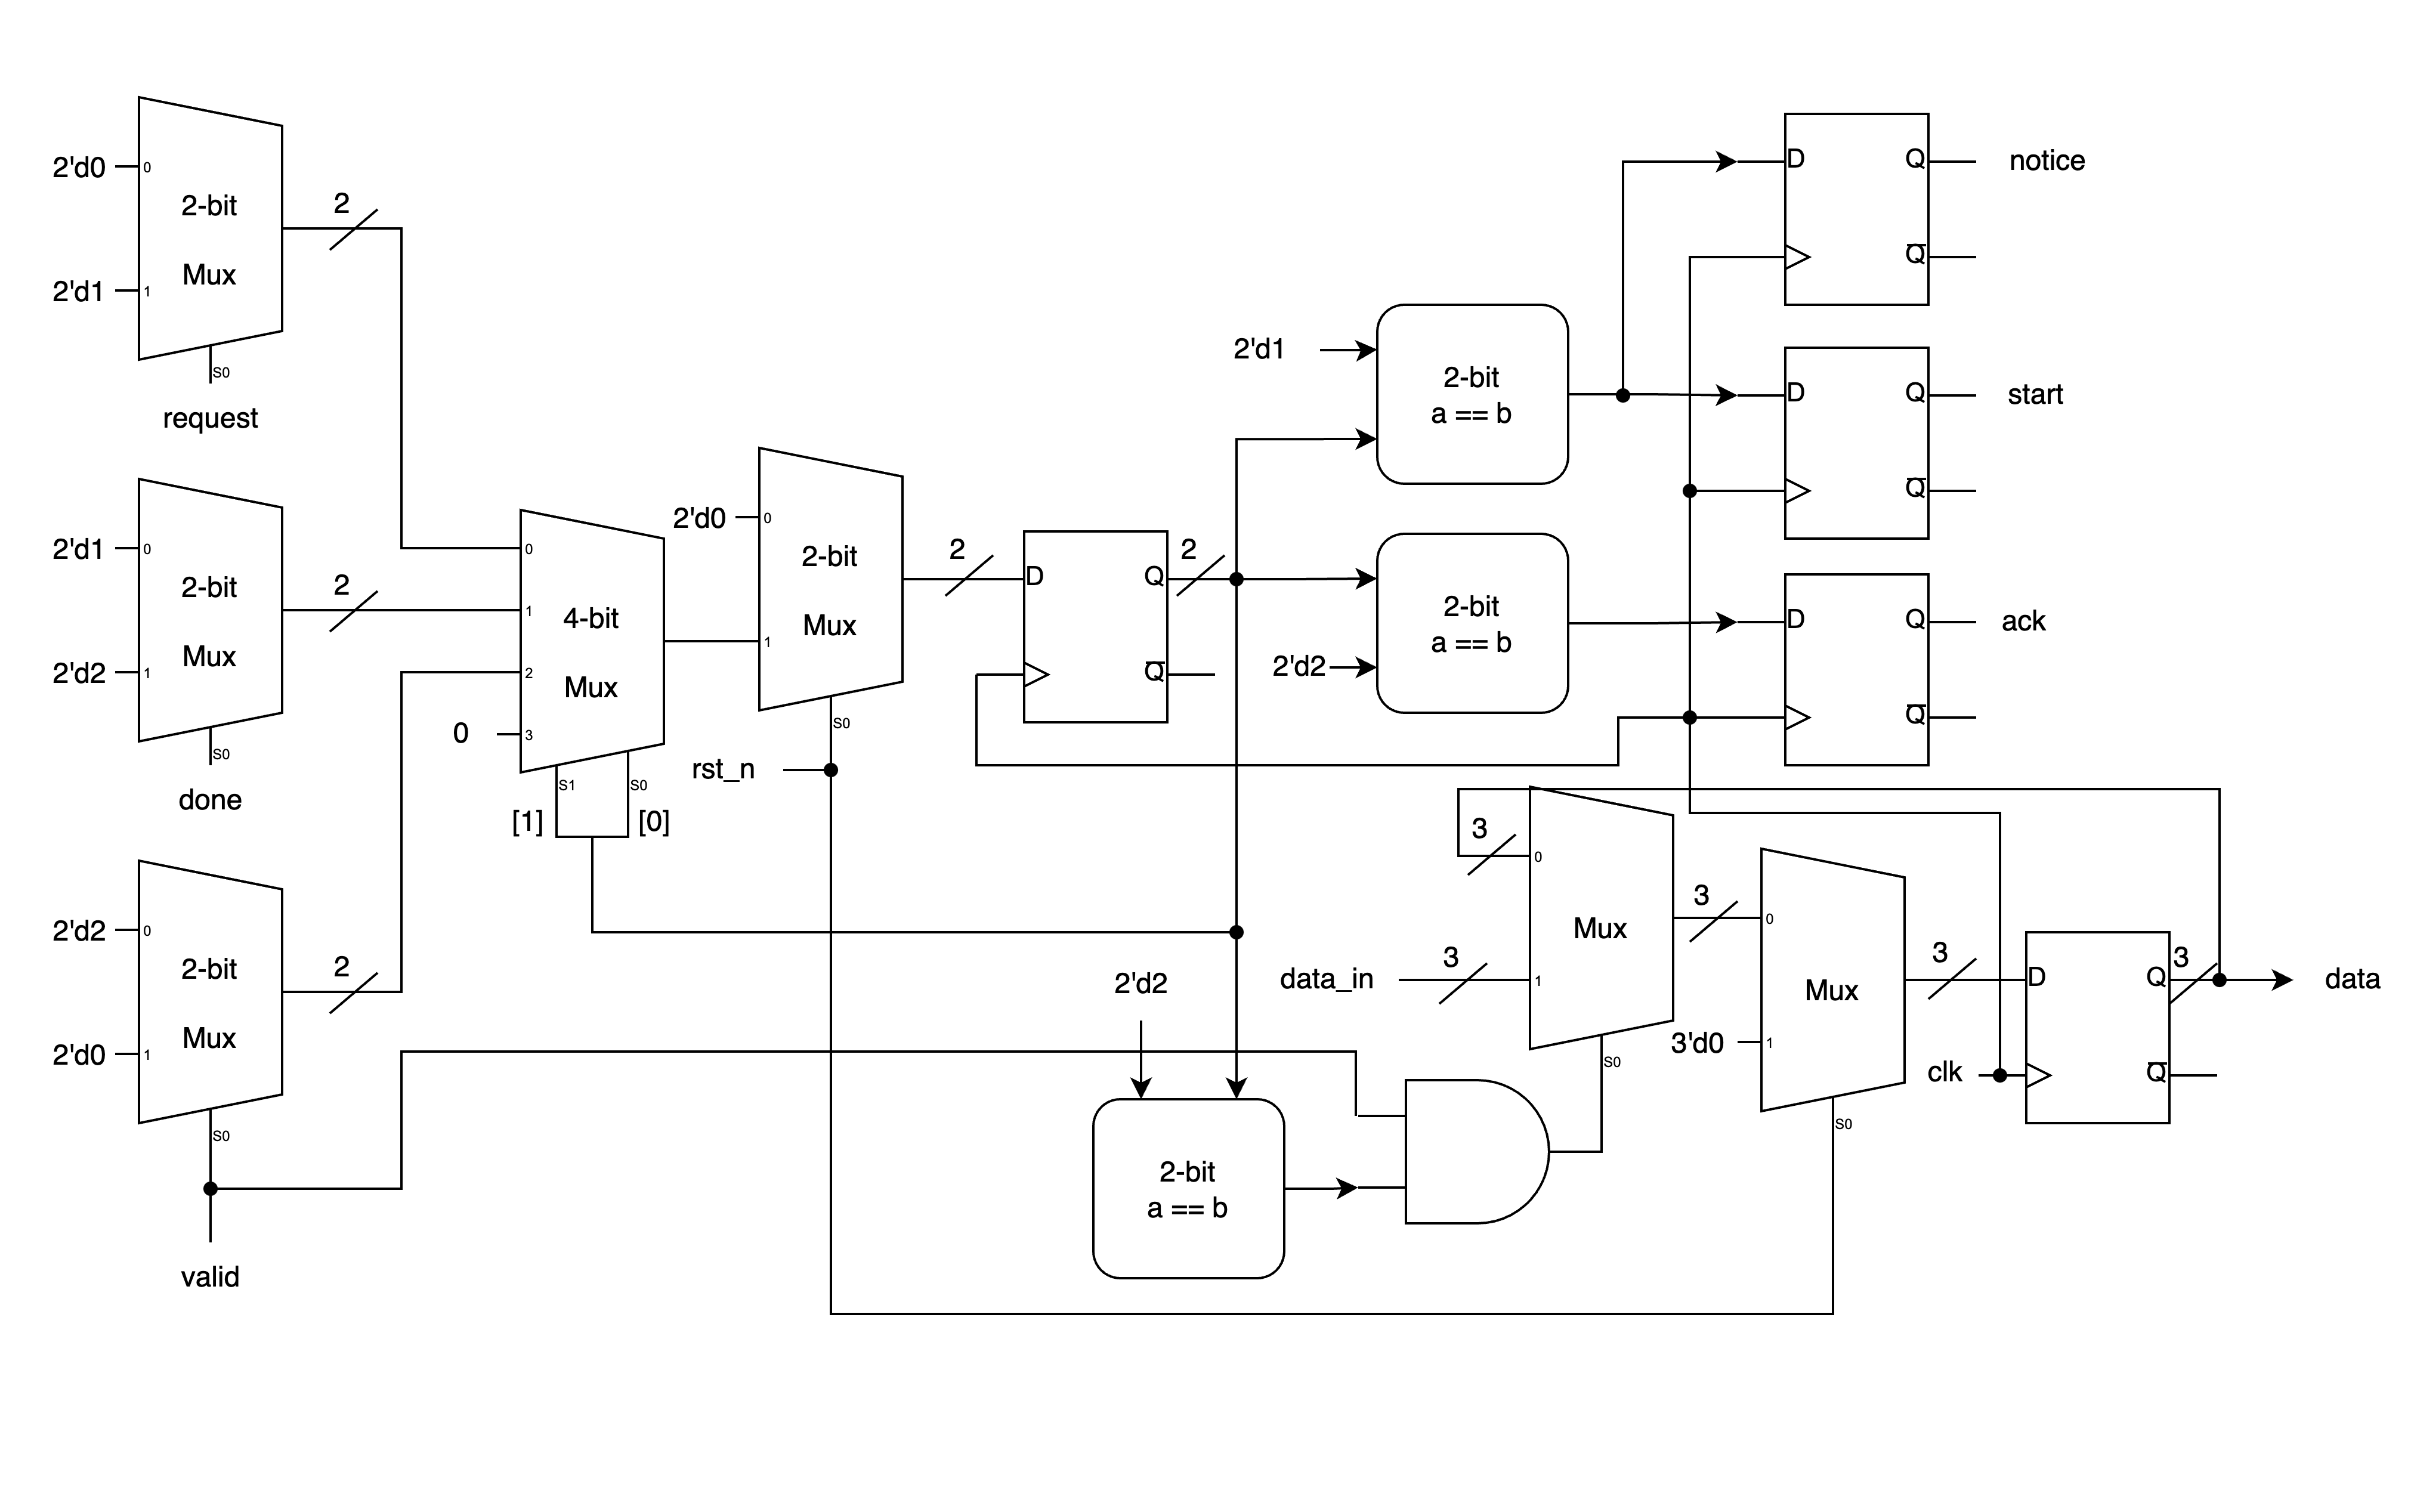
\includegraphics[width=0.9\textwidth]{./img/c2c-3.png}
  \caption{Q1 Slave Control Circuit}
  \label{fig:c2c-3}
\end{figure}

\newpage
\section{Slot Machine}

這題要在 FPGA 上實作使螢幕呈現往上的 777 動畫,板子上的 Top Button 為 Reset 訊號,\
Left Button 按下時要顯示往上的動畫,Right Button 按下時要顯示往下的動畫。

首先在原本的 sample code 上加入 Left Button 的 input(start\_up),\
當 start\_up 為 1 時表示要顯示一個往上的動畫,當 start 為 1 時表示要顯示一個往下的動畫。
\par
state\_control 處理完每幀畫面位置的 X\_v\_count 後,\
交給 mem\_addr\_gen 產生圖片與螢幕對應的正確記憶體位置,\
blk\_mem\_gen\_0 再根據輸出的 pixel\_addr 產生圖片 7 對應的 RGB,\
vga\_controller 則用於給予 mem\_addr\_gen 必要的輸入項,整體流程圖如下:

\begin{figure}[!h]
  \centering
  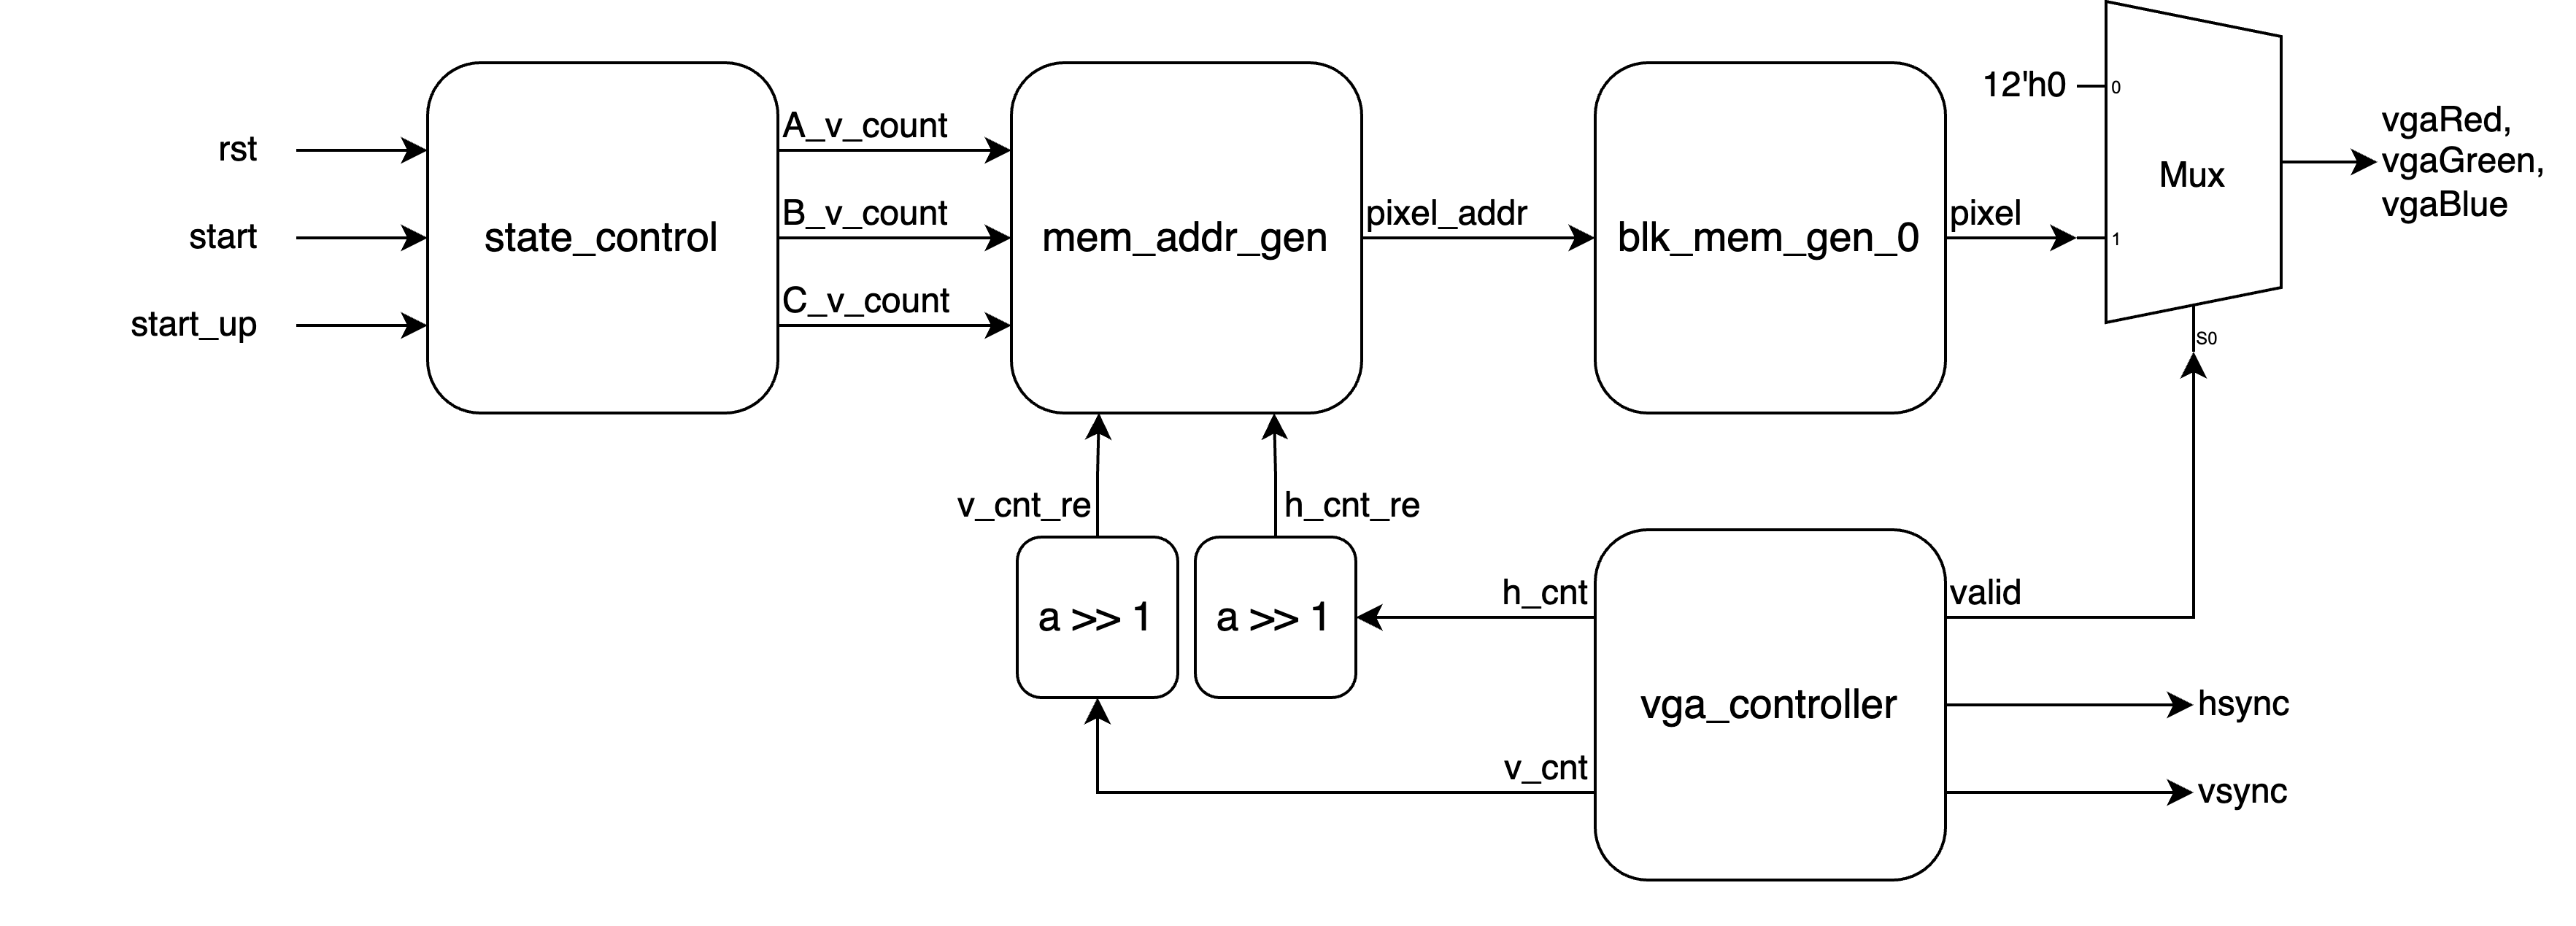
\includegraphics[width=0.9\textwidth]{./img/slot-1.png}
  \caption{Q2 Slot Machine FPGA block diagram}
  \label{fig:slot-1}
\end{figure}

\subsection{Motification}

在 state\_control 中,原先的 A\_to, B\_to, C\_to 在 counter 等於 0 時,\
透過 start 決定是否開始動畫,加入 start\_up 後,將 A\_to, B\_to, C\_to 修改成當 start\_up 為 1 時也會開始動畫。

(為了避免簡報過於冗長,後面以 X 替代 A, B, C)

\begin{figure}[!h]
  \centering
  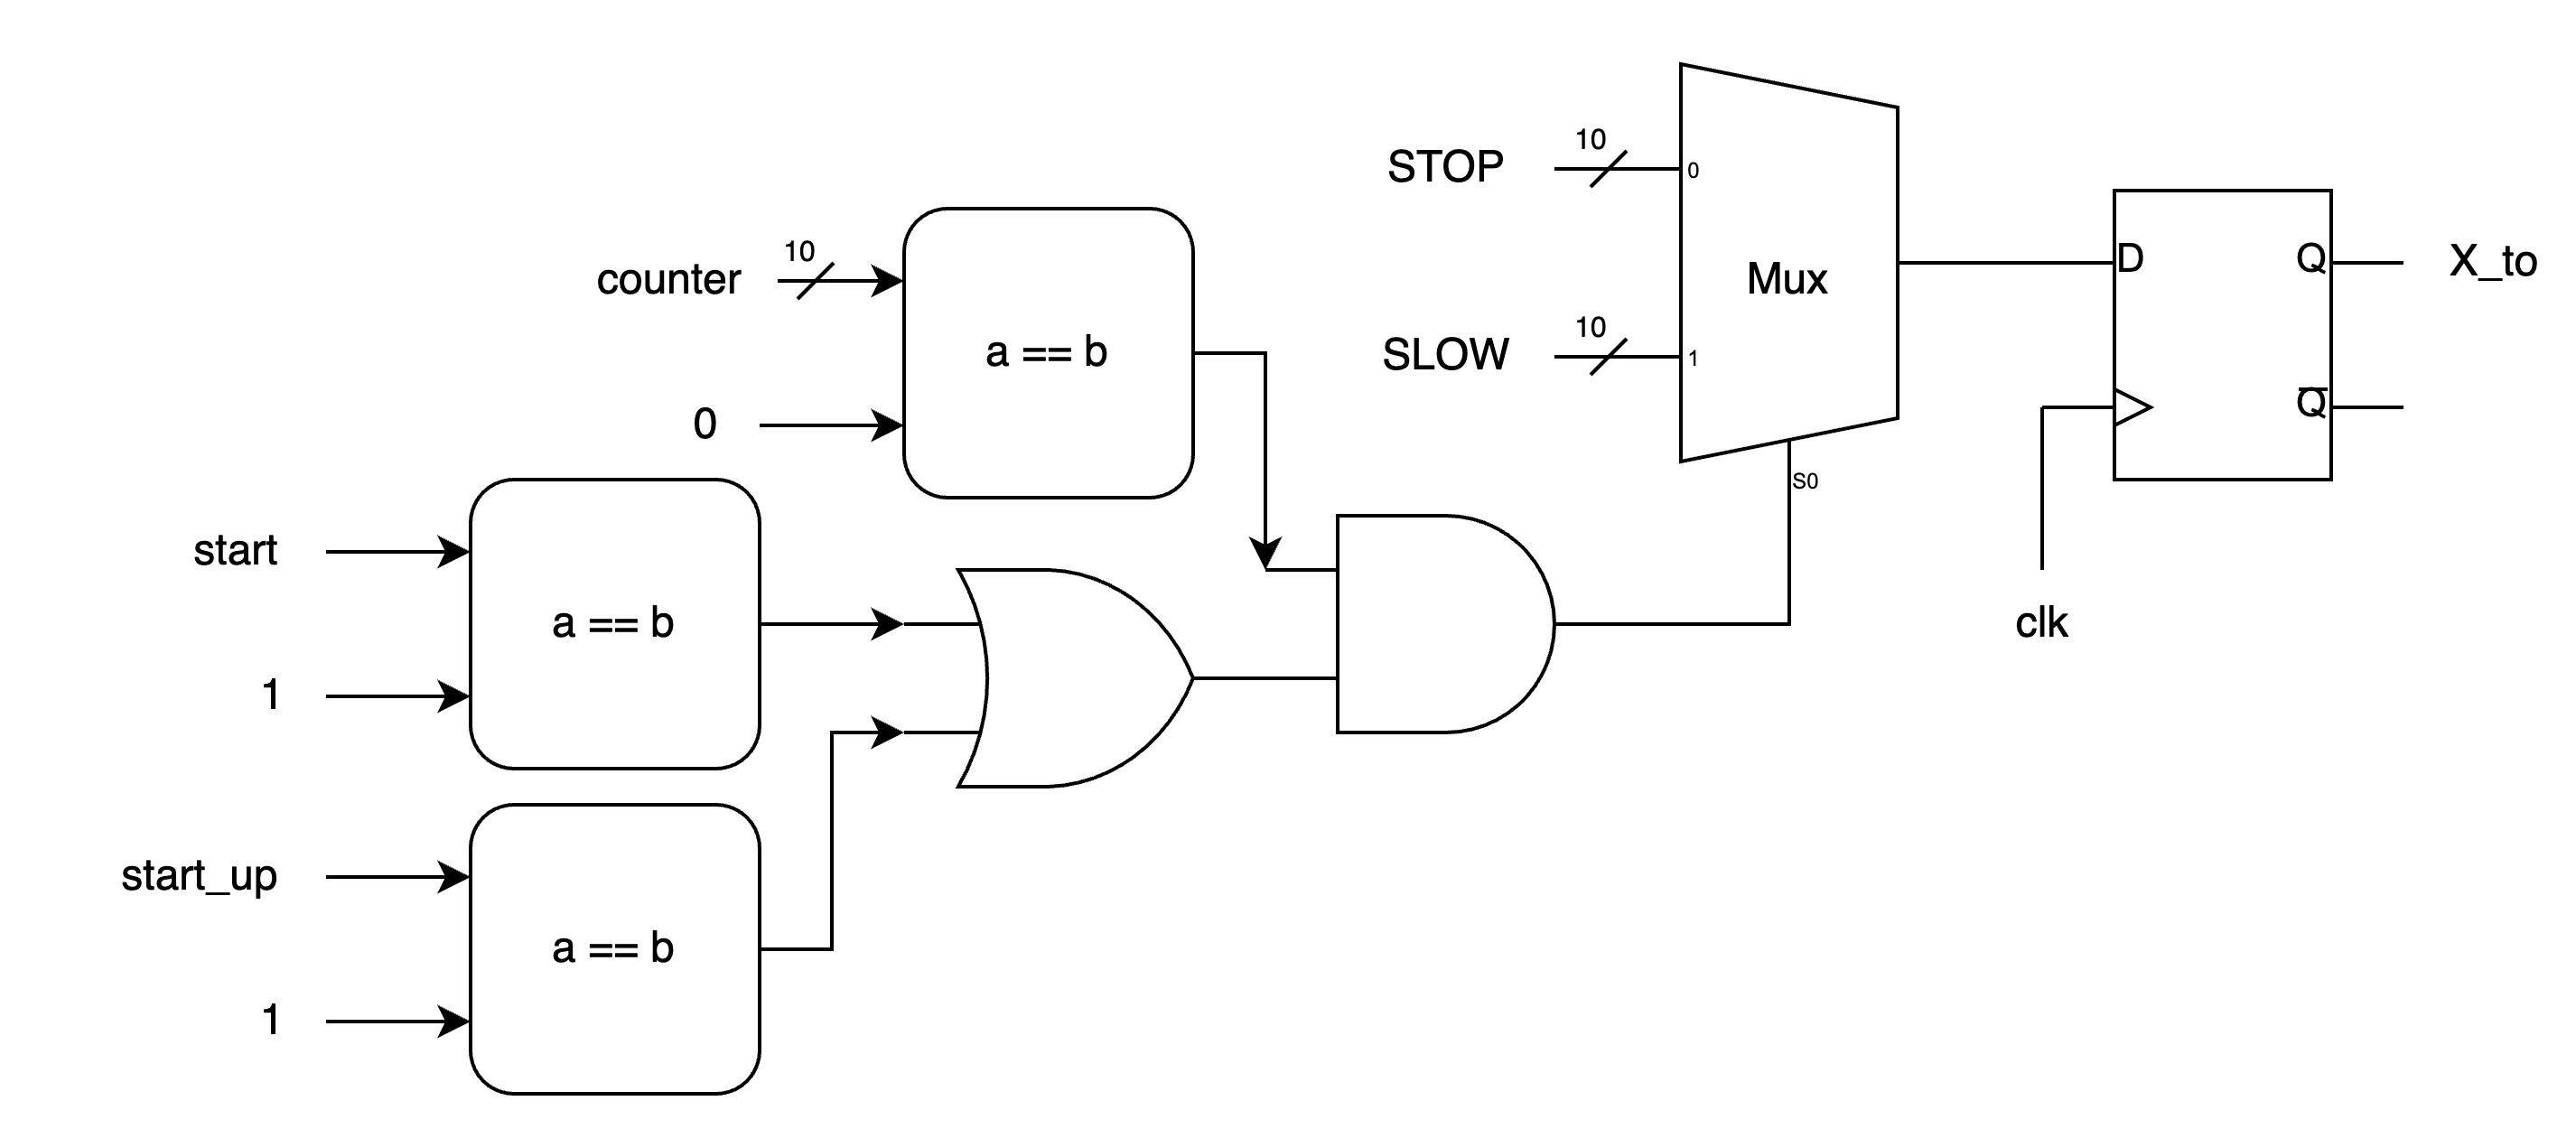
\includegraphics[width=0.9\textwidth]{./img/slot-2.png}
  \caption{Q2 Slot Machine X\_to Circuit}
  \label{fig:slot-2}
\end{figure}

對於 next\_counter,因為加入了 start\_up,將原本 (start==1'b0 \&\& counter==10'd0) \
修改為 (start==1'b0 \&\& start\_up==1'b0 \&\& counter==10'd0),\
使 start 和 start\_up 未按下並且 counter 為 0 時,讓 counter 歸 0 不再持續運作。
\par
為了使 start\_up 按下後不需要經過 reset,直接按下 start 也可以繼續運作,\
將 counter >= 10'd1000 的情況發生時,使 counter 歸 0。

\begin{figure}[!h]
  \centering
  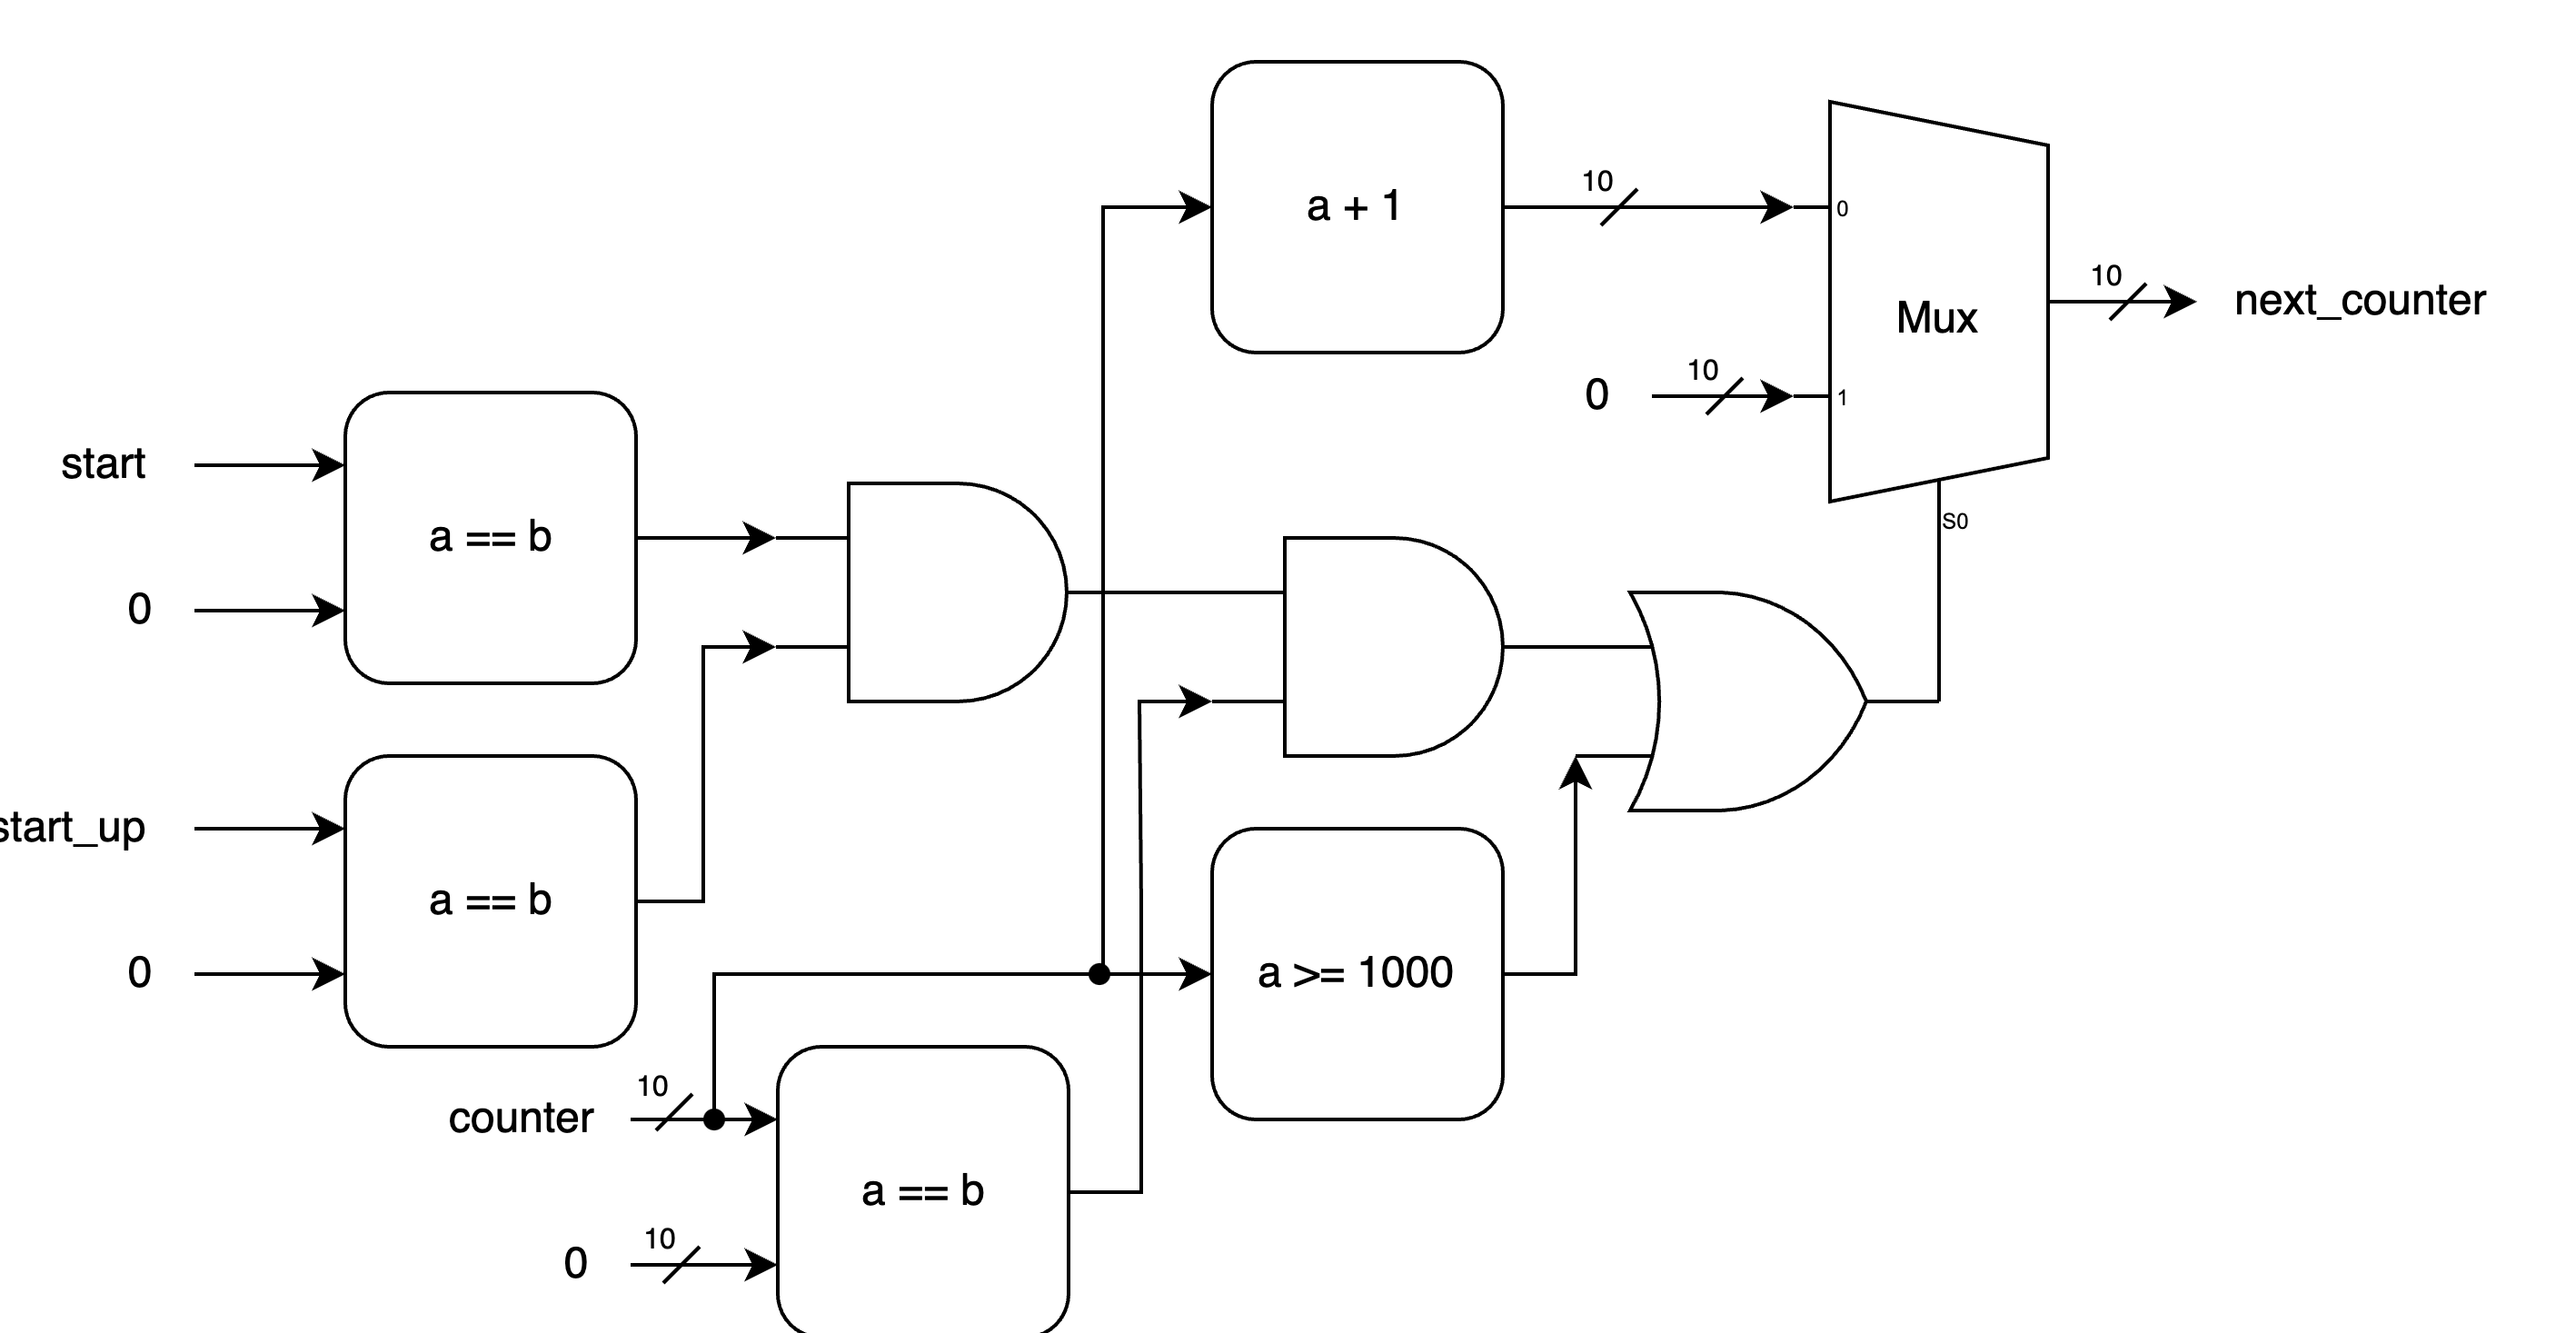
\includegraphics[width=0.8\textwidth]{./img/slot-3.png}
  \caption{Q2 Slot Machine next\_counter Circuit}
  \label{fig:slot-3}
\end{figure}

\newpage

我們加入一個 direction,當 counter 等於零且 start 被按下時,direction 設定為 0,\
且當 counter 等於零且 start\_up 被按下時,direction 設定為 1,其他情況 direction 維持原樣。

\begin{figure}[!h]
  \centering
  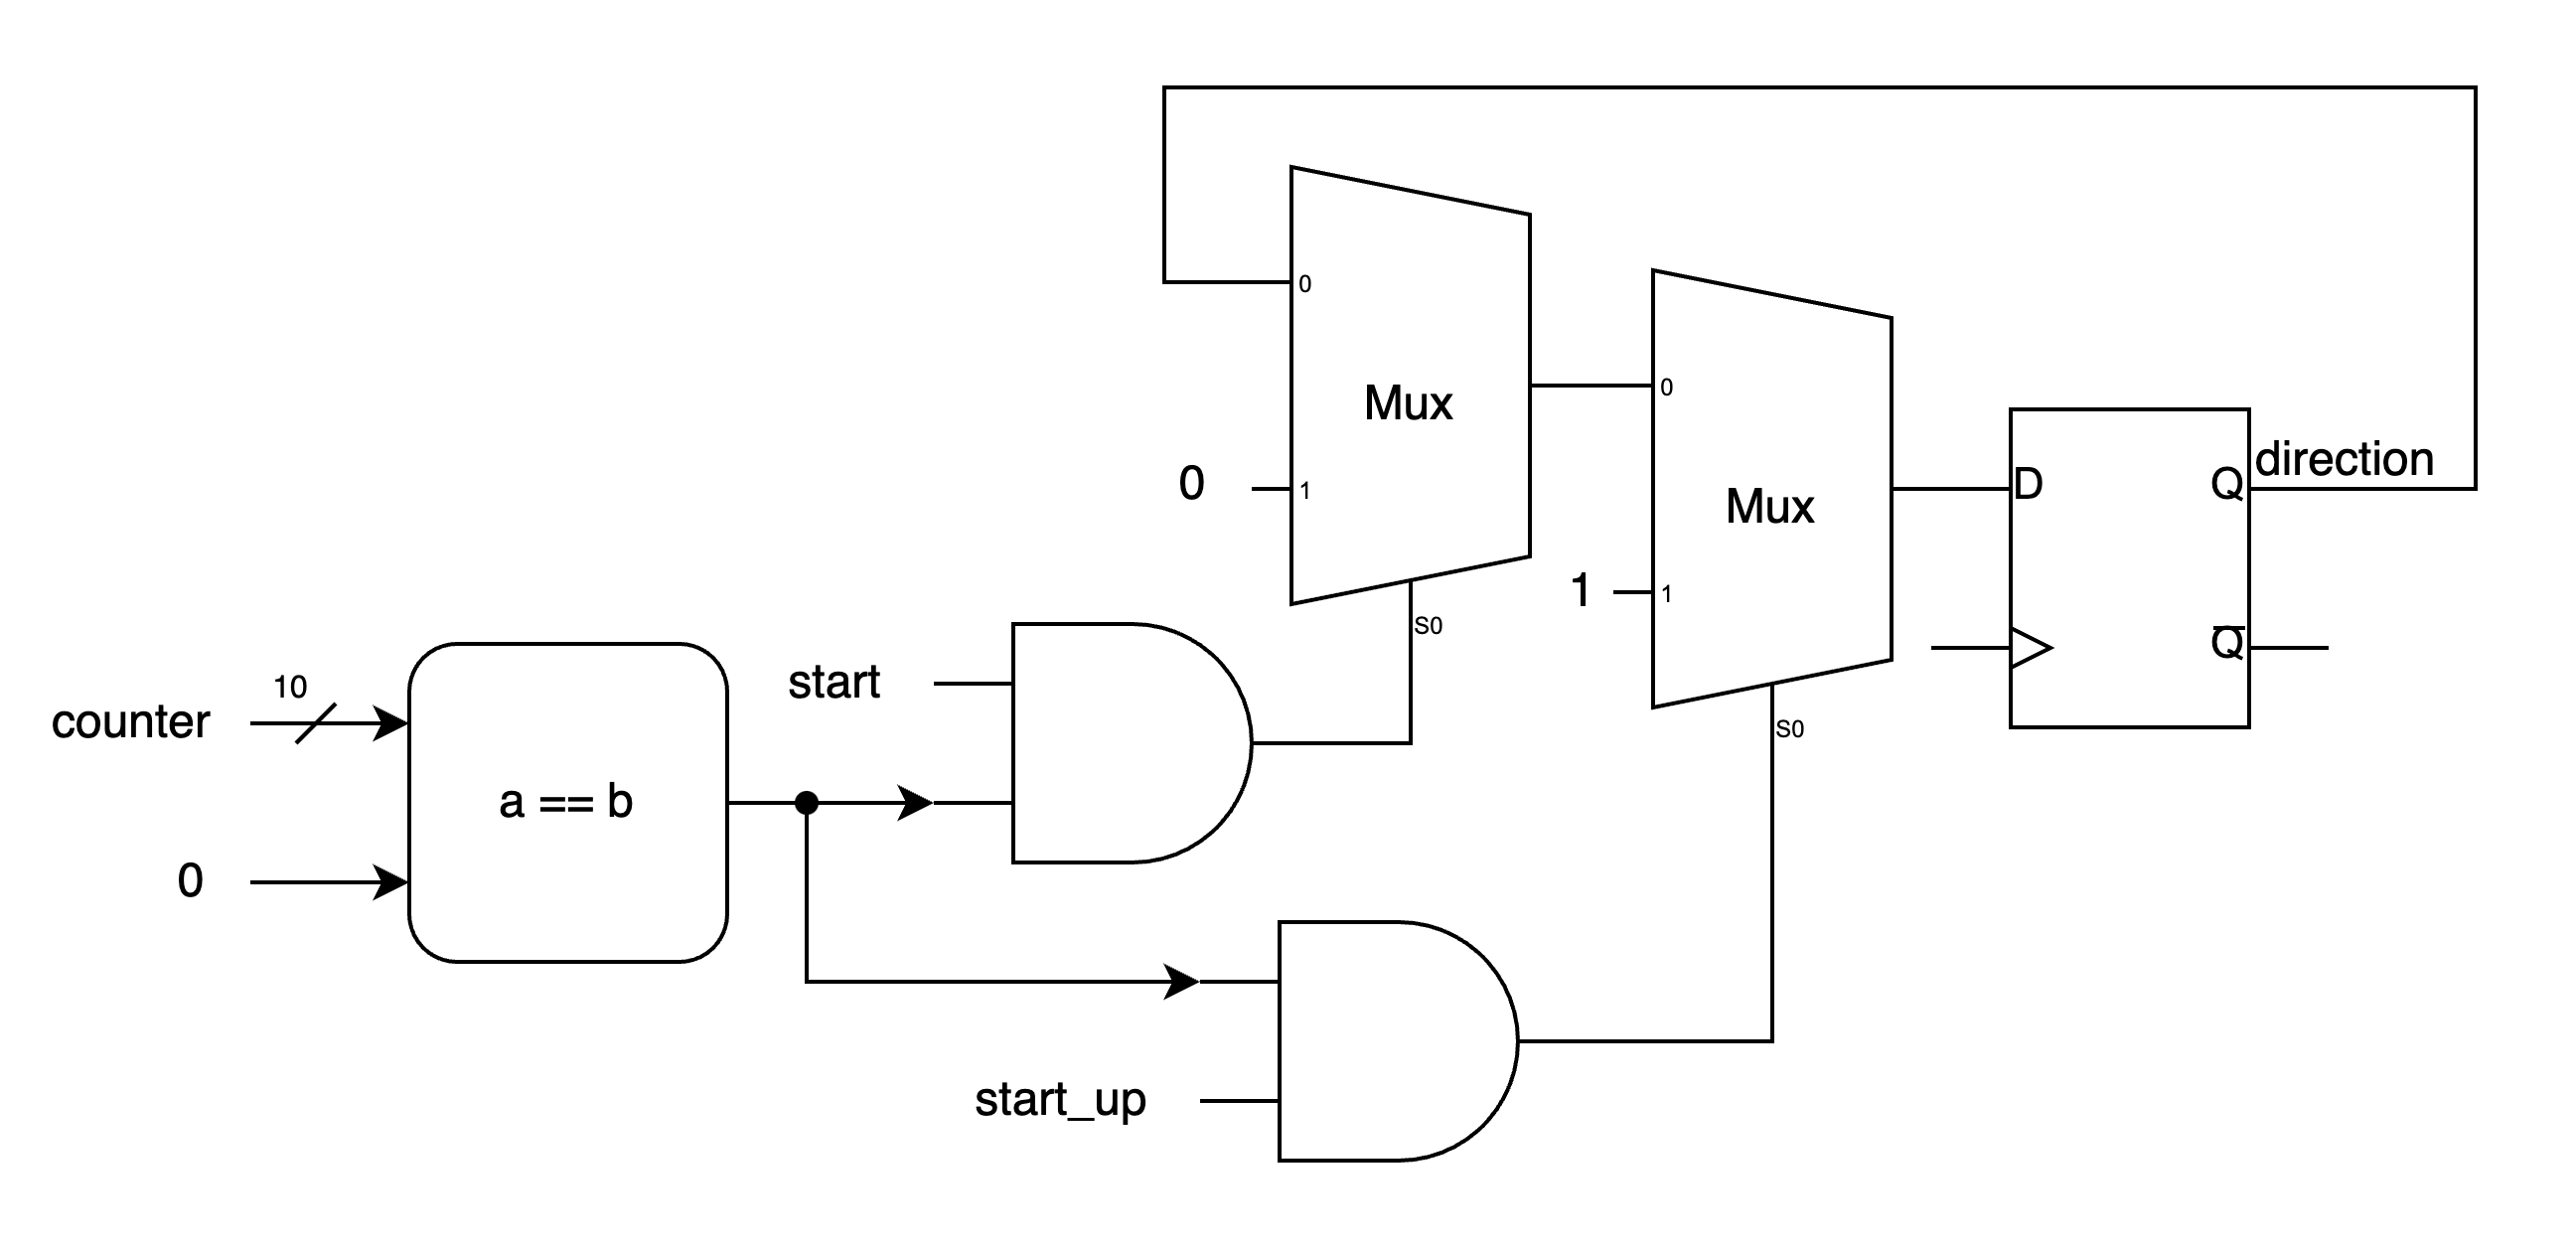
\includegraphics[width=0.8\textwidth]{./img/slot-4.png}
  \caption{Q2 Slot Machine direction Circuit}
  \label{fig:slot-4}
\end{figure}

接著新增了 up\_X\_v\_count 用來計算往上的 count,\
利用先前的 direction 變數用來判斷當下的\\ next\_X\_v\_count 會是往上還是往下的 count。

\begin{figure}[!h]
  \centering
  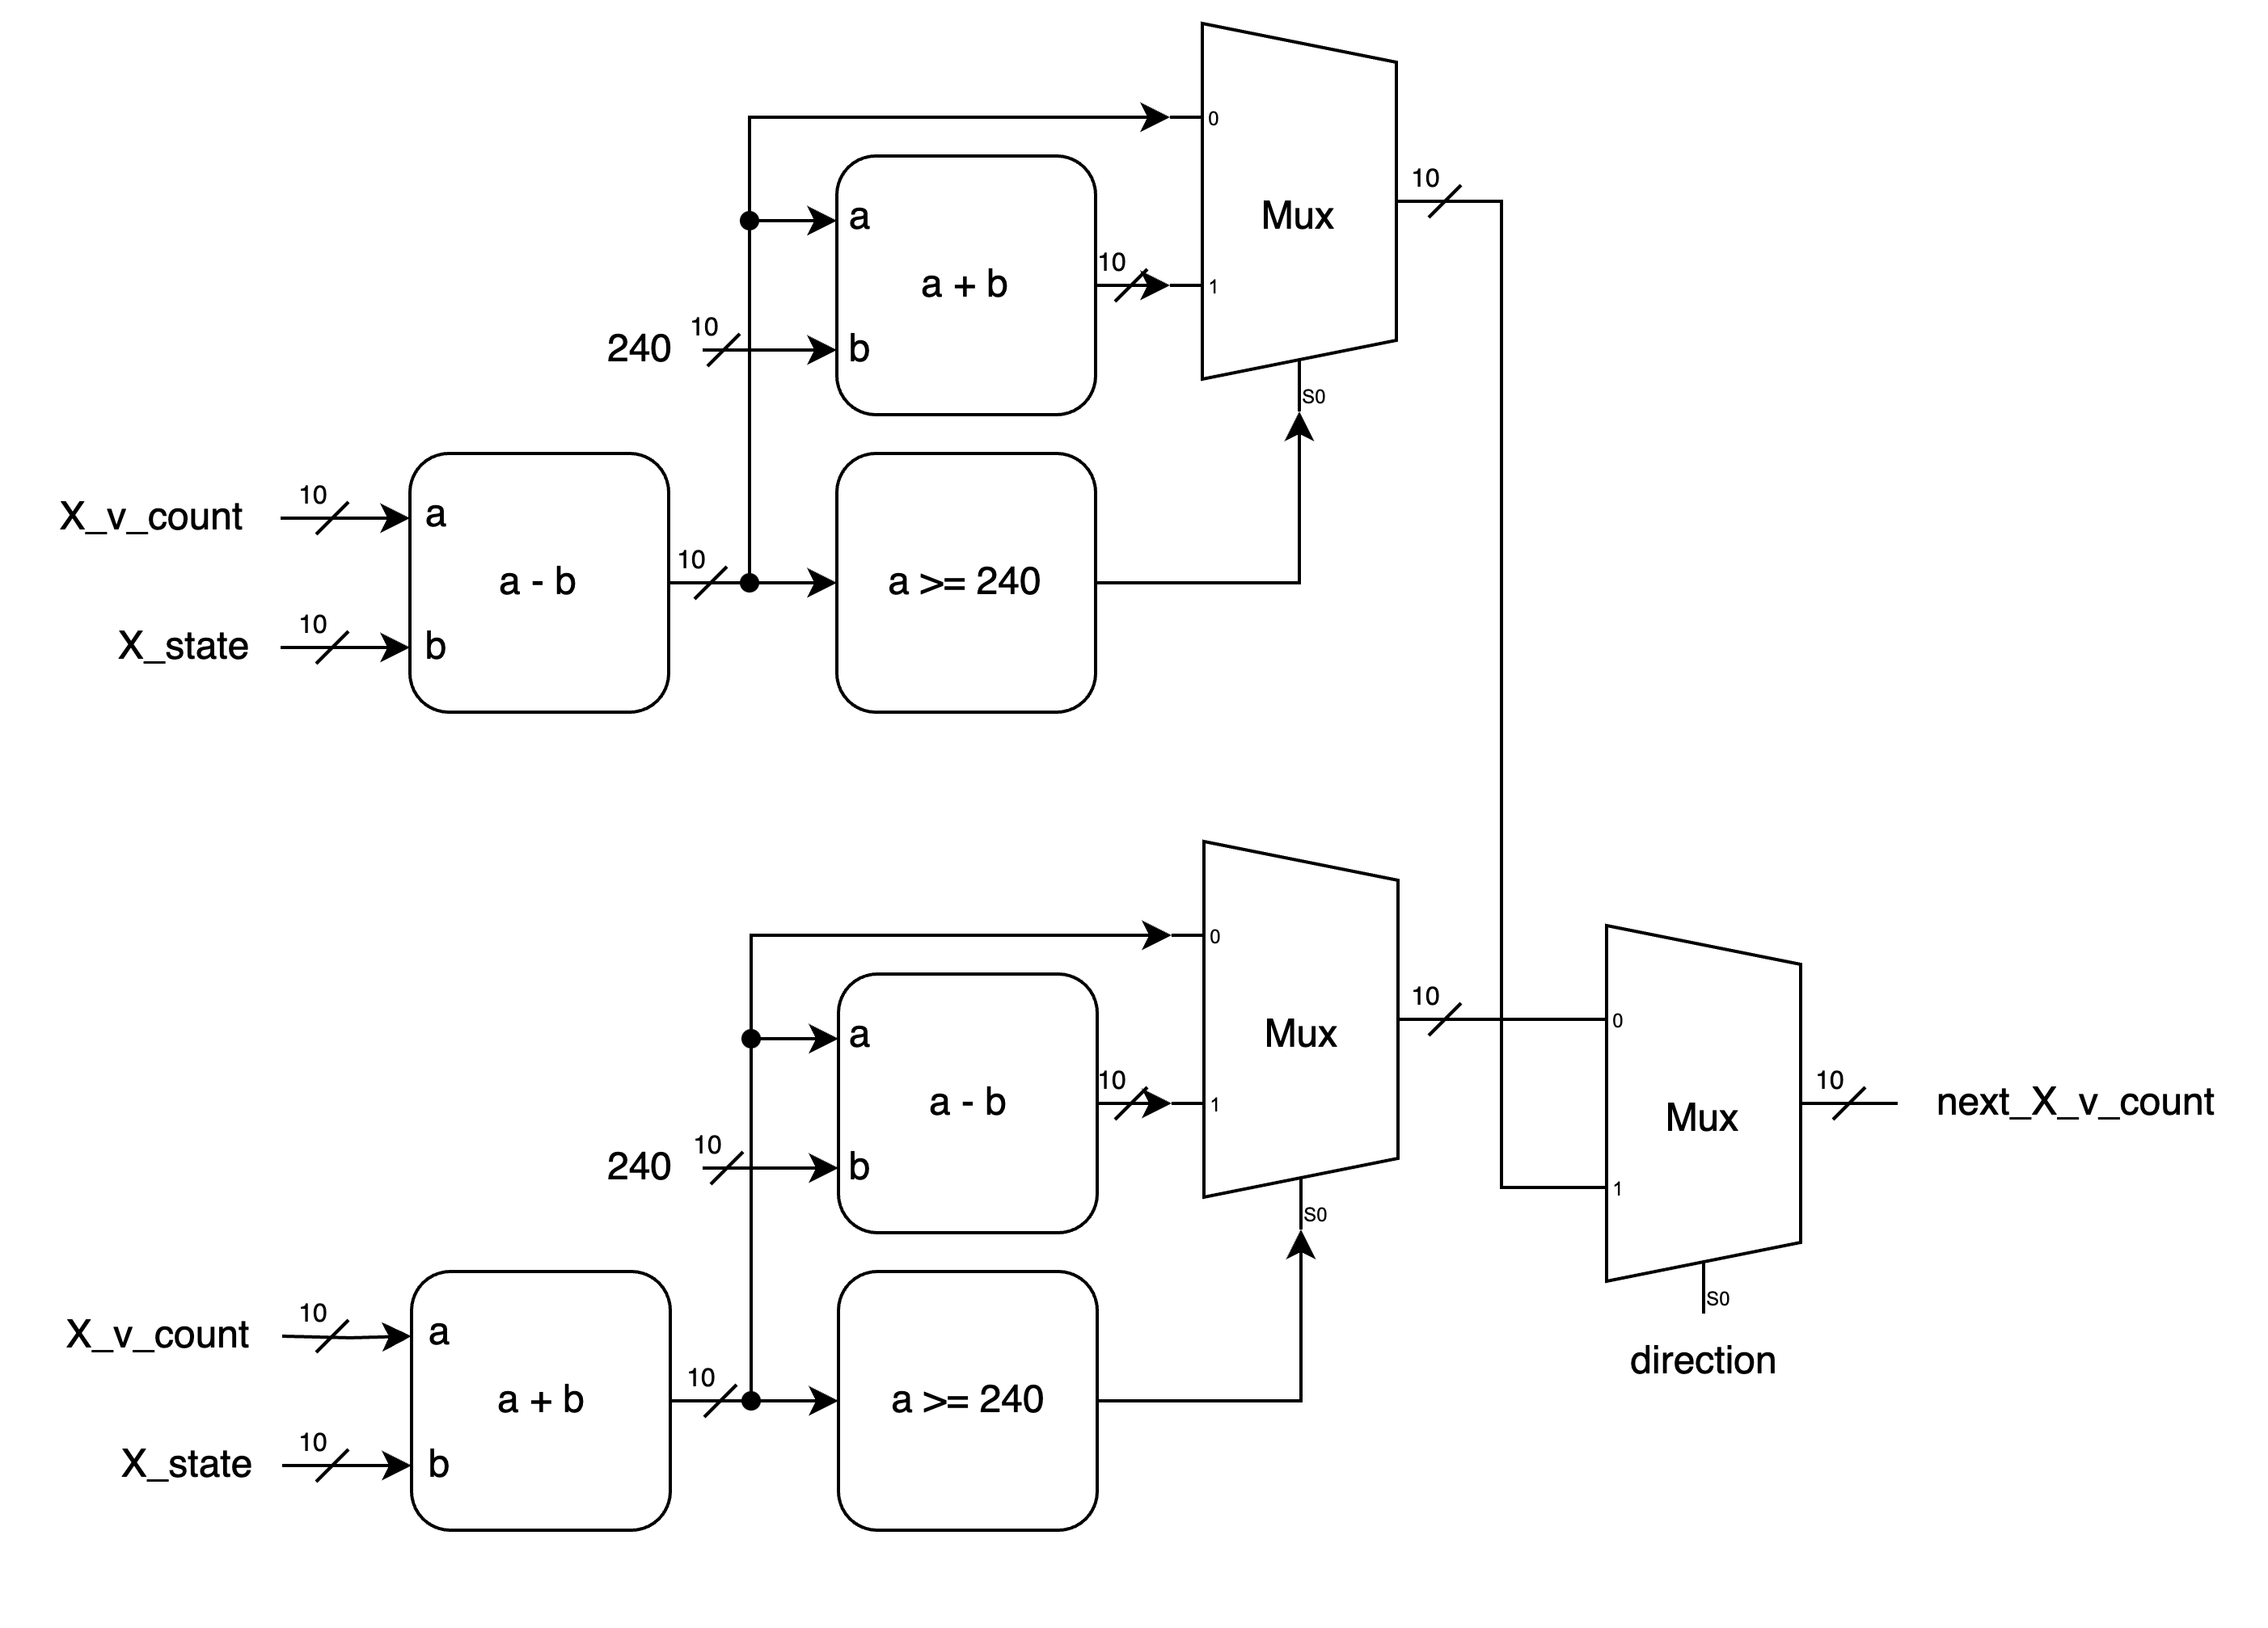
\includegraphics[width=0.9\textwidth]{./img/slot-5.png}
  \caption{Q2 Slot Machine up\_X\_v\_count Circuit}
  \label{fig:slot-5}
\end{figure}

\section{Car}

這部分我們需要使用 FPGA、超音波感應器、線路追蹤器以及馬達來組成一個自走車,\
使其能夠在寬度為 12 公分的白色賽道上自動行駛。

\subsection{Sonic}
超音波感應器的部分由四個 module 組成:sonic\_top, PosCounter, TrigSignal, div:

\subsubsection*{div}
將板子 100 MHz 的 clock 轉換為 1 MHz

\subsubsection*{TrigSignal}
產生 10 us 的 Trig 信號,週期為 10ms

\subsubsection*{PosCounter}
這個 module 會負責計算超音波回波的時間並轉換成距離。\
運作過程中分成了三個狀態:
\begin{itemize}
  \item S0: 等待回波開始,當偵測到 Echo 的 posedge 時,就會進到 S1
  \item S1: 計算回波時間,每個 clk cycle 會將 counter 加一,\
  直到偵測到 Echo 的 negedge,就會進到 S2
  \item S2: 計算距離,單位為 0.01 公分
\end{itemize}

\subsubsection*{sonic\_top}
接收其他 module 計算出來的距離,判定如果距離小於 40 公分,就輸出停止訊號。\
不過由於資電館疑似有不乾淨的東西,導致超音波感應器在某些地方會偵測到不存在的物體,\
因此額外加了一個 $\texttt{enable\_stop}$ 訊號,\
使其能夠透過板子上的開關來決定是否要開啟超音波感應器的功能。

\newpage

\subsubsection*{Block Diagram}

\begin{figure}[h!]
  \centering
  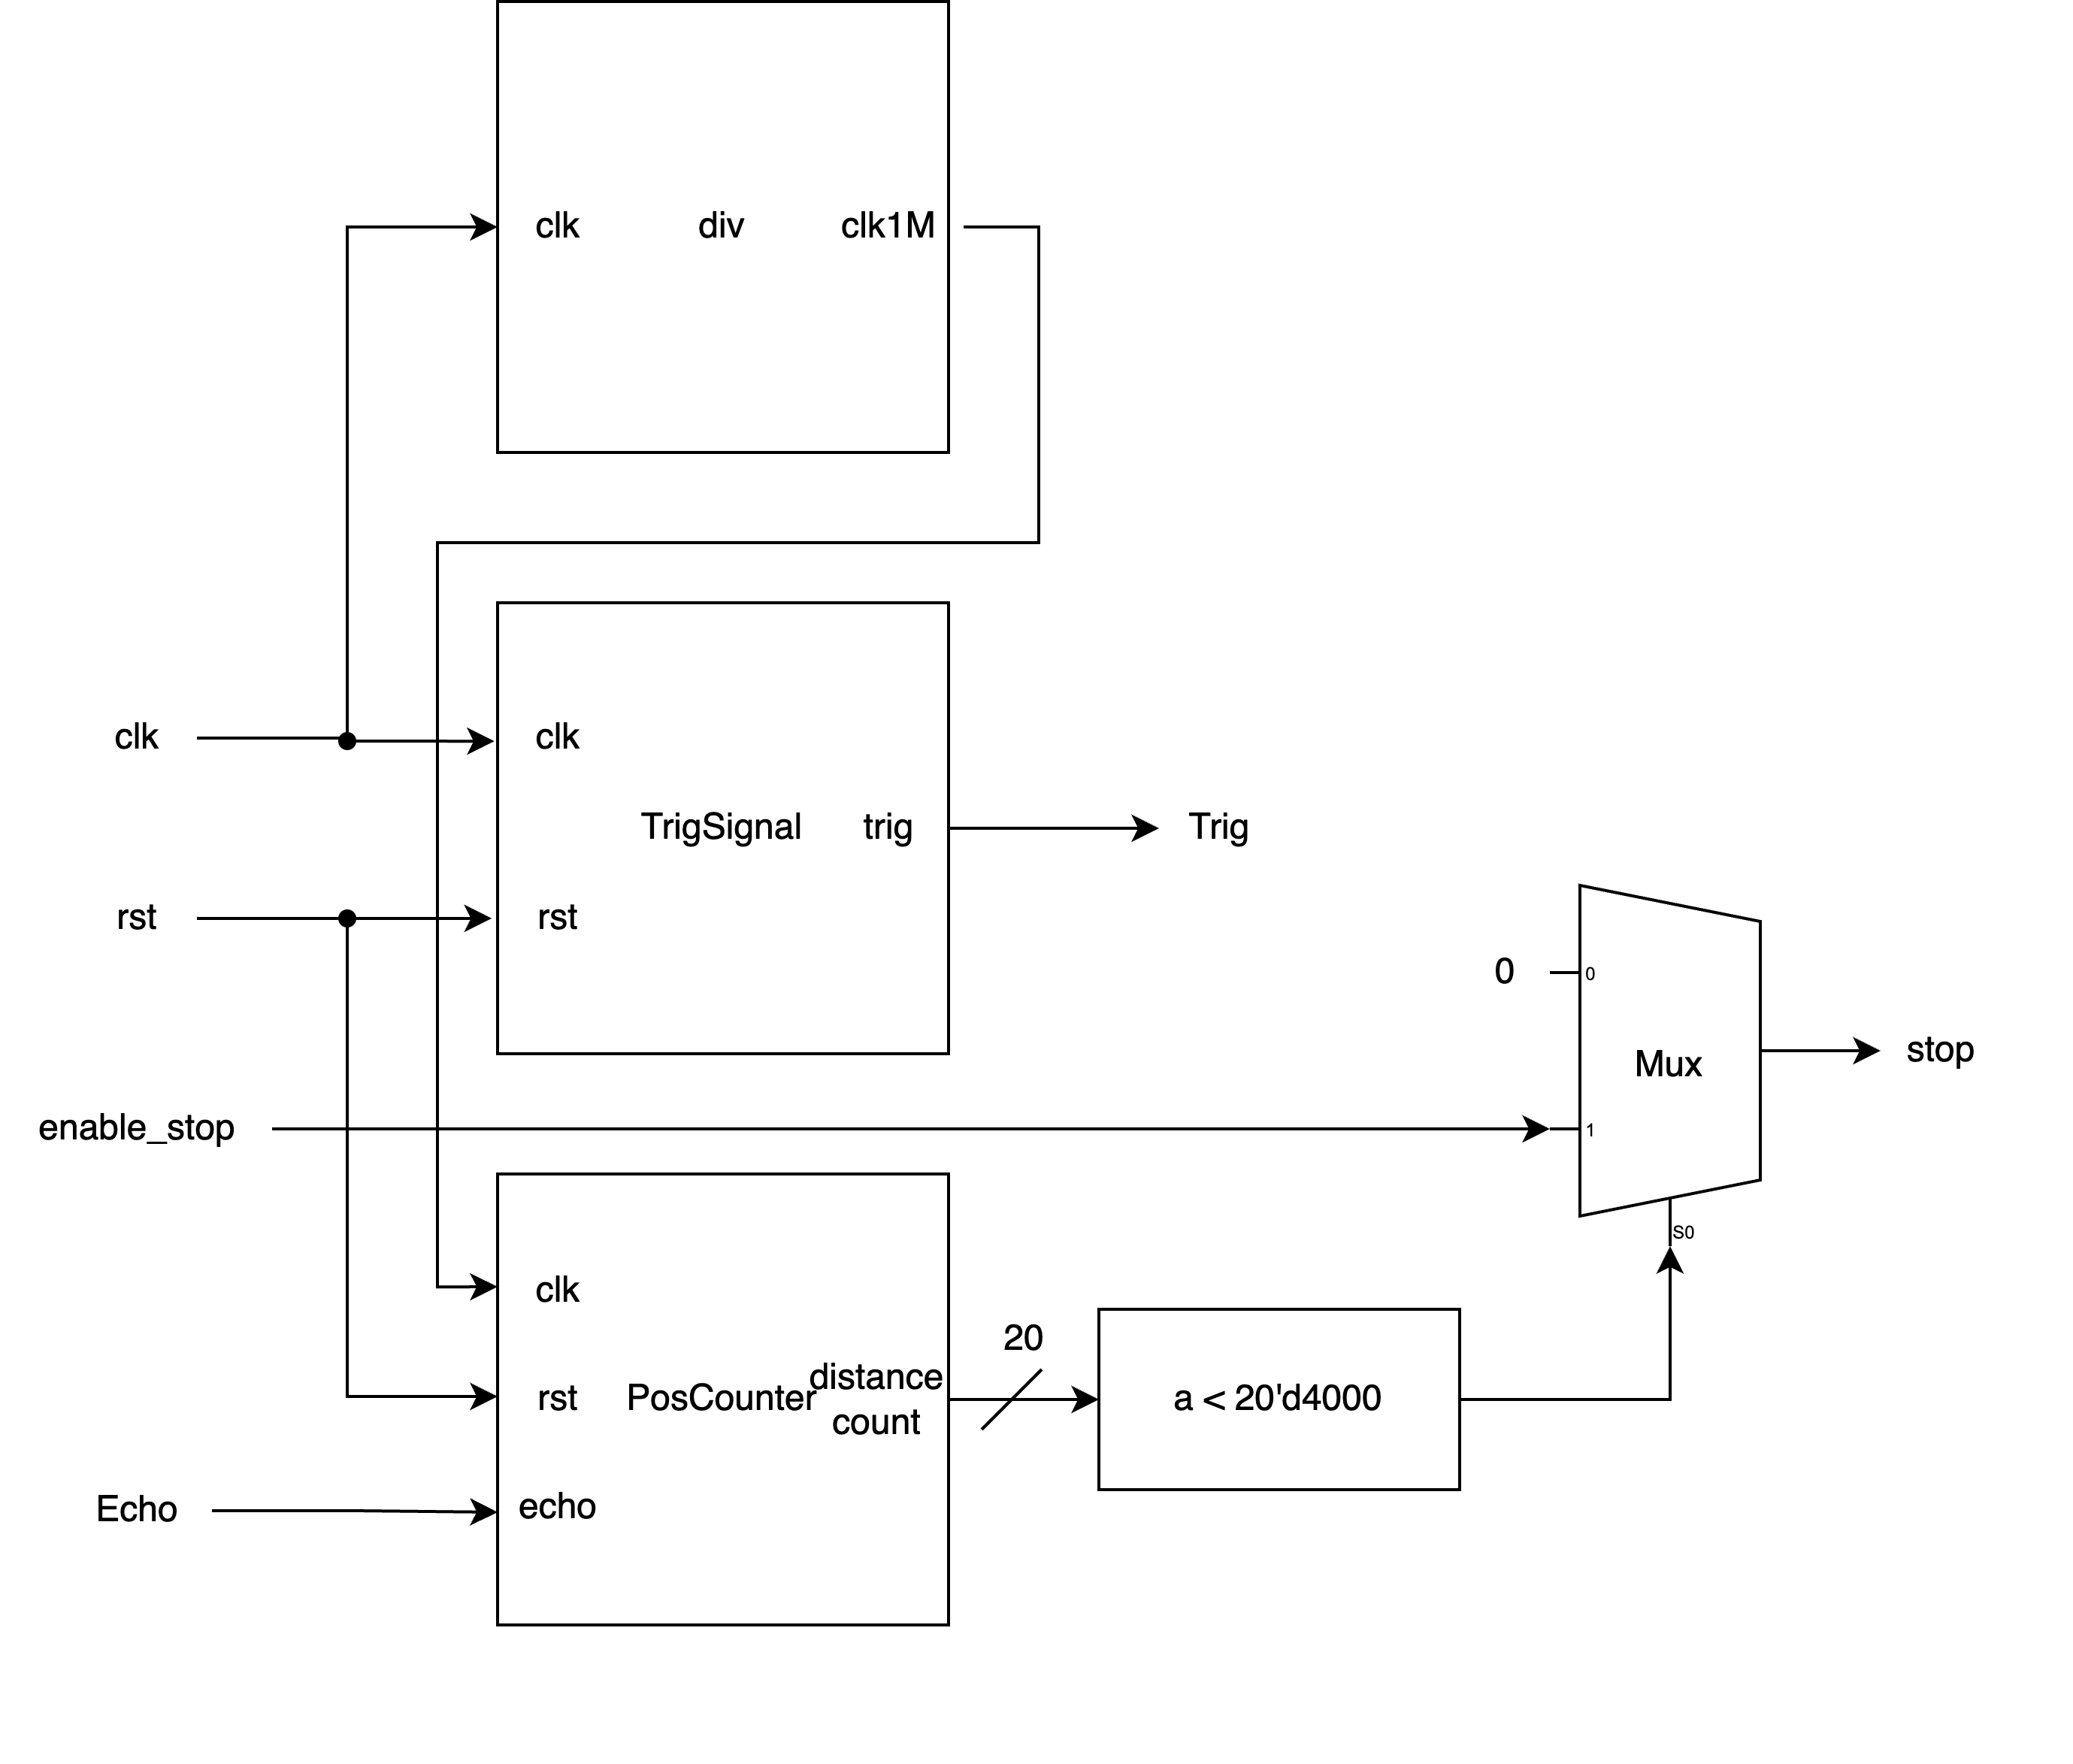
\includegraphics[width=0.9\textwidth]{./img/car-1.png}
  \caption{Sonic}
  \label{fig:sonic}
\end{figure}

\subsection{Tracking Strategy}

我們利用三個 bit 的 state 來表示感應器的狀態,\
state[2] 代表 left, state[1] 代表 middle, state[0] 代表 right,\
針對不同的策略調整馬達的運轉方向,而無論如何,馬達的速度都設定為 1023(最大值):

\subsubsection*{111}
這代表三個感應器都偵測到黑線,此時車子會直行。

\subsubsection*{001}
這代表車子已經向左偏移了不少,此時左輪會往前,右輪會往後,使車子更快的向右轉。

\subsubsection*{011}
如果車子是從 $111$ 的狀態轉變過來的,則右輪會停止,左輪會往前,使車子緩慢的向右轉。\
反之如果車子是從 $001$ 的狀態轉變過來的,那代表還沒有完全轉回來,則會繼續保持左輪往前、右輪往後的狀態。

\subsubsection*{100, 110}
這兩個狀態與 $001, 011$ 相似,只是方向相反。

\subsubsection*{其它}
保持不變。

\begin{figure}[!h]
  \centering
  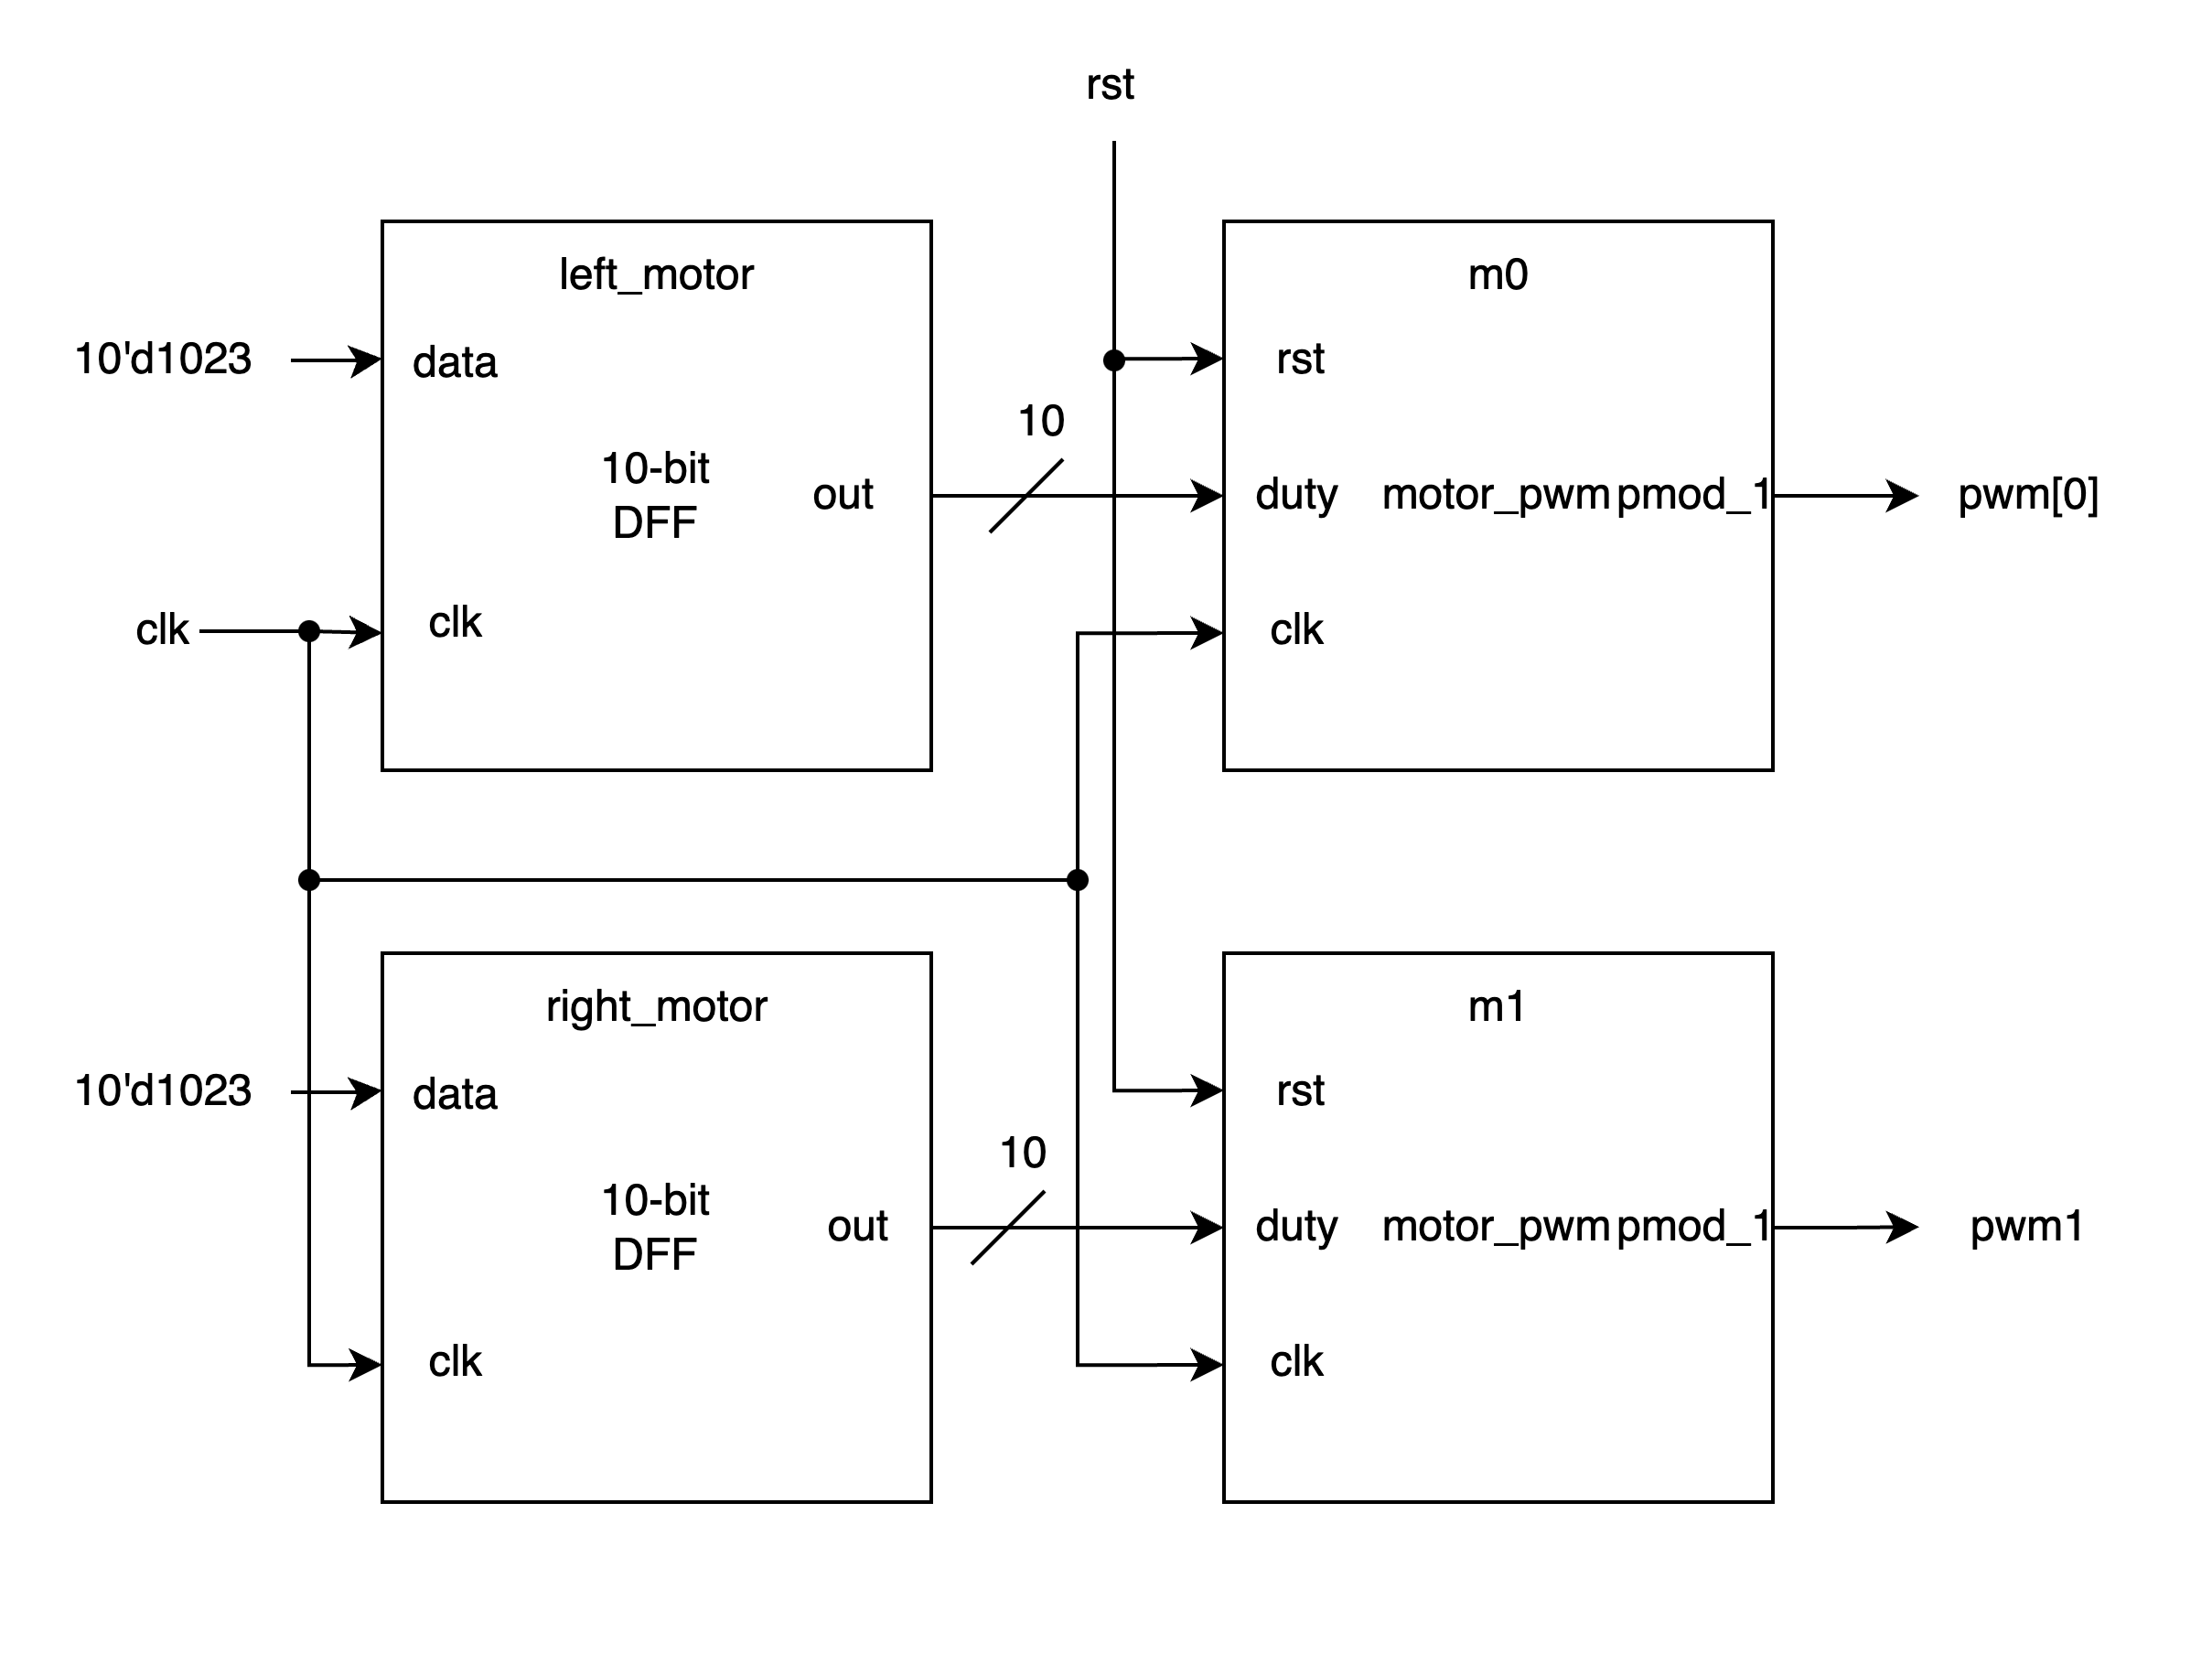
\includegraphics[width=0.7\textwidth]{./img/car-2.png}
  \caption{Tracking Strategy}
  \label{fig:tracking}
\end{figure}

\newpage

\subsection{Overall}

\begin{figure}[h!]
  \centering
  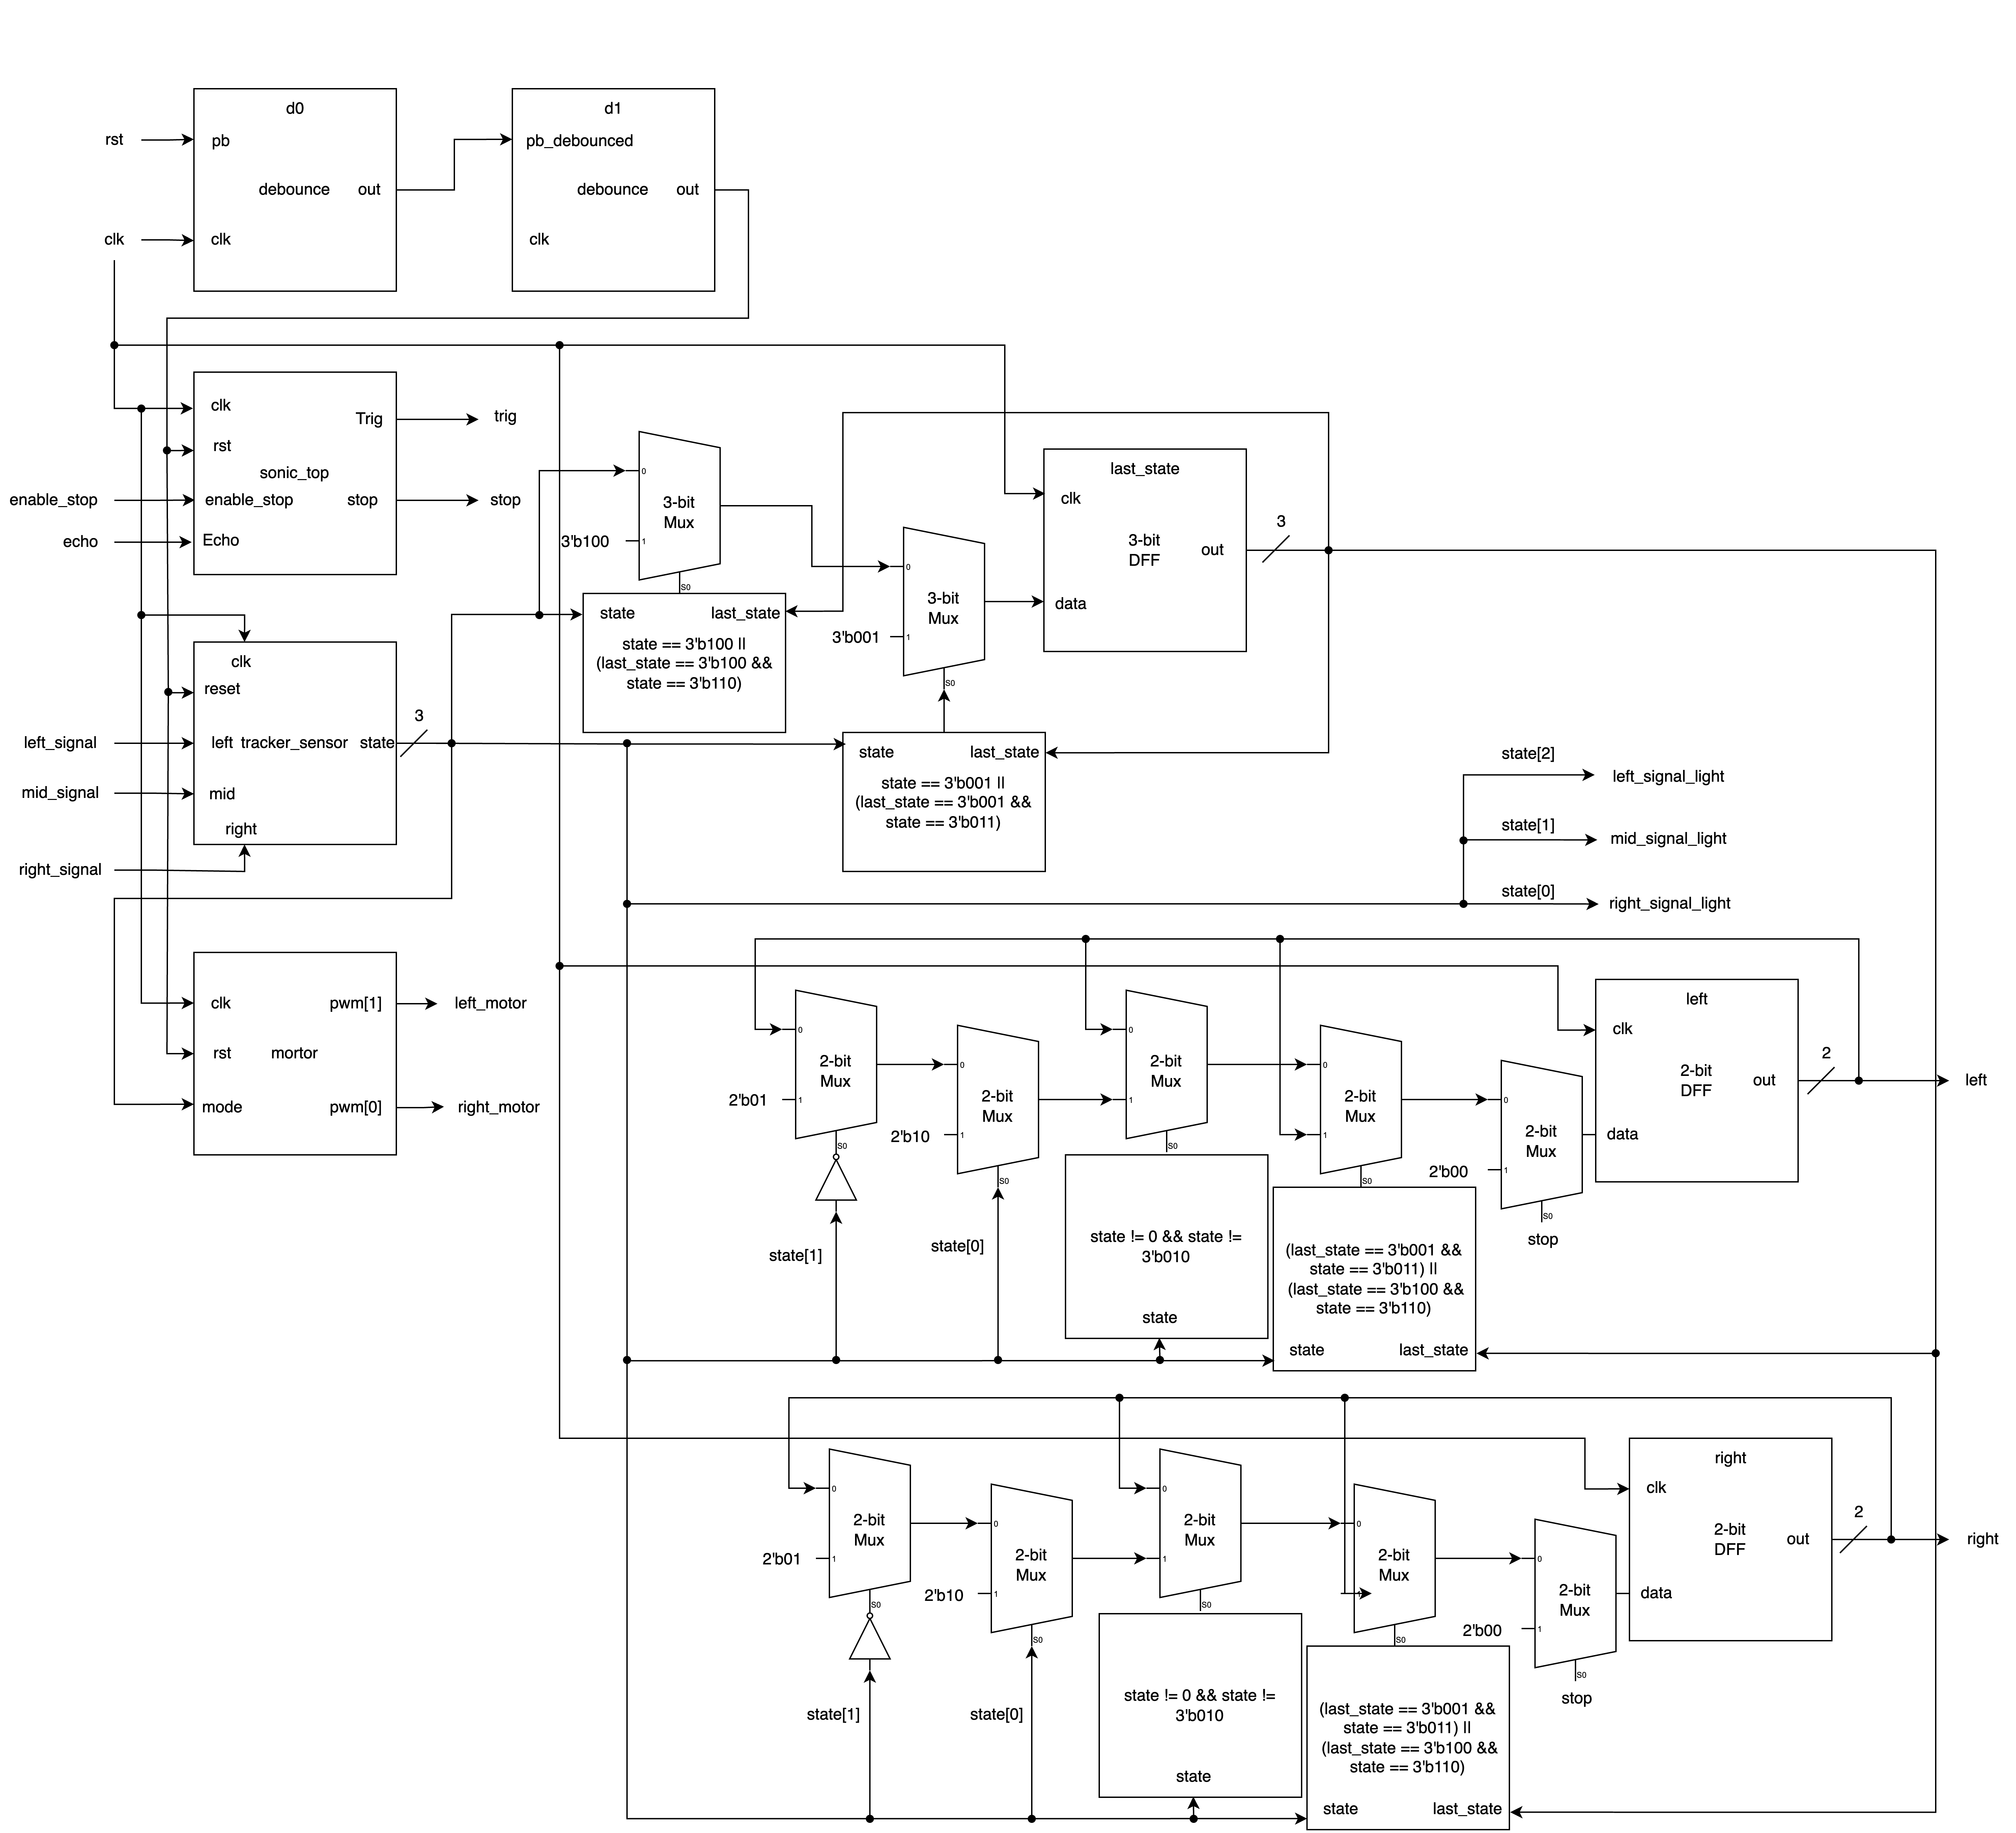
\includegraphics[width=0.9\textwidth]{./img/car-3.png}
  \caption{Overall}
  \label{fig:overall}
\end{figure}

\newpage
\newpage

\subsection{What We Have Learned}

\begin{itemize}
  \item 學習到了如何實際應用 Handshaking protocol 在兩塊 FPGA 板上做數據傳輸,以及將圖片動畫透過 VGA 傳輸到電腦螢幕上顯示
  \item 超音波感應器的原理以及距離計算
  \item 如何使用線路追蹤器來控制馬達的運轉方向
  \item 如何設計一個簡單的 state machine 來控制車子的運行
\end{itemize}

\subsection{分工}
\begin{itemize}
  \item 陳克盈:Car
  \item 蔡明妡:Chip-to-Chip, Slot Machine
\end{itemize}

\end{document}


